\documentclass[14pt]{extarticle}


\usepackage[utf8]{inputenc}
\usepackage[T2A]{fontenc}      %% 2
\usepackage[english,russian]{babel}    %% 3



\usepackage[square,numbers]{natbib}
\usepackage{setspace}
\usepackage{amssymb}
\usepackage{lipsum}

\usepackage{graphicx}
\usepackage{amsmath}
\usepackage{marvosym}

\usepackage{subfig}
\usepackage{float}
\usepackage{booktabs}
\usepackage{xcolor}
\usepackage{hyperref}
\usepackage{comment}
\definecolor{linkcolor}{HTML}{000000} % цвет ссылок
\definecolor{urlcolor}{HTML}{000080} % цвет гиперссылок
\hypersetup{pdfstartview=FitH,  linkcolor=linkcolor,urlcolor=urlcolor, colorlinks=true}
\renewcommand{\baselinestretch}{1.5}
\bibliographystyle{abbrvnat}
\renewcommand{\bibsection}{\center{\section*{СПИСОК ИСПОЛЬЗОВАННЫХ ИСТОЧНИКОВ}}}

\usepackage{geometry}
	\geometry{papersize={21.0 cm, 29.7 cm}}
	\geometry{top=20mm}
	\geometry{bottom=20mm}
	\geometry{left=30mm}
	\geometry{right=20mm}
	

\usepackage{tocloft} % подключение модуля управления содержанием, списком рисунков и таблиц...
        

%\onehalfspacing
\renewcommand{\baselinestretch}{1.5}

\begin{document}
 
\def\contentsname{Содержание}

\newpage

%\renewcommand{\baselinestretch}{1.5}

\begin{titlepage}
\begin{center}
%\large
ФЕДЕРАЛЬНОЕ ГОСУДАРСТВЕННОЕ БЮДЖЕТНОЕ ОБРАЗОВАТЕЛЬНОЕ УЧРЕЖДЕНИЕ ВЫСШЕГО ОБРАЗОВАНИЯ МОСКОВСКИЙ ГОСУДАРСТВЕННЫЙ УНИВЕРСИТЕТ\\ имени М.~В.~ЛОМОНОСОВА

\vspace{0.5cm}

ФИЗИЧЕСКИЙ ФАКУЛЬТЕТ

\vspace{0.5cm}

КАФЕДРА КВАНТОВОЙ ЭЛЕКТРОНИКИ
\vfill

МАГИСТЕРСКАЯ ДИССЕРТАЦИЯ\\[5mm]

{\bfseries «АППАРАТНО ЭФФЕКТИВНЫЙ АНЗАЦ ДЛЯ ВАРИАЦИОННЫХ КВАНТОВЫХ АЛГОРИТМОВ»}
\bigskip

\end{center}

%\vfill
\vspace{0cm}

\newlength{\ML}
\settowidth{\ML}{«\underline{\hspace{0.9cm}}» \underline{\hspace{2cm}}}
\hfill\begin{minipage}{0.48\textwidth}
\begin{center}
Выполнил студент\\ 227мм академической группы\\ Жбанников Станислав Олегович\\
\hskip-1em\vtop{\vskip.1cm\hsize=2.9in \hrulefill}

\linespread{1}
{\small \centering подпись студента\par}
\linespread{1.5}
\end{center}
\end{minipage}%

%\vspace{1.5cm}
\vfill

\hfill\begin{minipage}{0.48\textwidth}
\begin{center}
Научный руководитель:\\ к.ф.-м.н., с.н.с. \\Сайгин Михаил Юрьевич\\
\hskip-1em\vtop{\vskip.1cm\hsize=2.9in \hrulefill}

\linespread{1}
{\small \centering подпись научного руководителя\par}
\linespread{1.5}
\end{center}
\end{minipage}%

%\vspace{1.5cm}
\vfill

\begin{minipage}{0.45\textwidth}
\begin{flushleft}
Допущен к защите 25.05.2022
\\Зав. кафедрой \hskip0.5em\vtop{\vskip.1cm\hsize=1.4in \hrulefill}\\
\linespread{1}
{\small \centering {подпись зав. кафедрой}\par}
\linespread{1.5}
\end{flushleft}
\end{minipage}%\hfill%

\vspace*{\fill}
{\centering Москва\\ 2022 \par}

\end{titlepage}

\setcounter{page}{2}

\newpage

%\renewcommand{\baselinestretch}{1.3}
%\linespread{1.3}

\setcounter{page}{2}

\begin{center}
\tableofcontents
\end{center}

\newpage

%\linespread{0.5}

\begin{center}
\section*{ВВЕДЕНИЕ}
\end{center}

\addcontentsline{toc}{section}{ВВЕДЕНИЕ}



\qquad Квантовые вычисления как самостоятельная область науки появились в 1980-х годах благодаря идее проводить вычисления на квантовых системах, значительно ускоряя  некоторых трудоёмкие для классического компьютера вычисления \cite{feynman1982simulating}. С того времени было предложено множество теоретических квантовых алгоритмов, позволяющих получить полиномиальное, а в определённых случаях экспоненциальное ускорение в сравнении с известными классическими алгоритмами при наличии универсального квантового компьютера. К наиболее известным квантовым алгоритмам можно отнести алгоритм Шора \cite{Shor}, позволяющий получить экспоненциальное ускорение для задачи факторизации числа и алгоритм Гровера \cite{Grover}, дающий квадратичное ускорение поиска по неструктурированной базе данных.

\qquad Параллельно с теоретическими открытиями развивались и сами технологии квантовых компьютеров. На сегодняшний день разработано множество подходов к физической реализации квантовых компьютеров, таких как преобразования над системами фотонов \cite{RevModPhys.79.135}, холодных атомов/ионов  в ловушках \cite{PhysRevA.66.032309}, квантовых точек \cite{PhysRevA.57.120} или сверхпроводящих цепей \cite{PhysRevB.68.064509}. Каждый из перечисленных подходов имеет свои преимущества, при этом ни одна из существующих технологий не позволяет реализовать универсальный квантовый компьютер ввиду ограничений на максимальный размер квантовой системы и её полностью запутанной подсистемы, а так же наличии ошибок при реализации преобразований. Доступные в настоящее время квантовые устройства способны выполнять преобразования с некоторым уровнем ошибок на небольших квантовых системах. Их принято называть шумными квантовыми устройствами среднего размера (в англоязычной литературе Noisy Intermidiate Scale Quantum NISQ) \cite{Preskill2018quantumcomputingin}. 

\qquad Прикладное использование таких квантовых алгоритмов, как алгоритм Шора или алгоритм Гровера требует недоступных для NISQ устройств ресурсов. Таким образом для практического использования существующих технологий, а так же устройств, которые предположительно появятся в ближайшем будущем, наиболее перспективными представляются гибридные алгоритмы, где часть операций выполняется на классическом компьютере и лишь подзадачи, сложные для классической обработки выполняются на квантовом устройстве. Важным классом гибридных квантово-классические алгоритмов являются вариационные квантовые алгоритмы ВКА (в англоязычной литературе variational quantum algorithms VQA) \cite{Cerezo_2021} основанны на принципе вариации параметров квантовой схемы. ВКА включают в себя различные группы алгоритмов, такие как вариационный квантовый алгоритм решения уравнений на собственные значения операторов ВКС (Variational Quantum Eigensolver англ. VQE) \cite{VQE_review}, квантовый приблизительный оптимизационный алгоритм КПОА (Quantum Approximate Optimization Algorithms англ. QAOA) \cite{QAOA}, Квантовые нейронные сети КНН (в англоязычной литературе quantum neural networks QNN) \cite{KAK1995259}.

\qquad Характеристики ВКА тоже зависят от ограничений, накладываемых квантовыми устройствами. Чтобы улучшить эти характеристики необходимо эффективно использовать физические возможности квантовых устройств. Для этого используются аппаратно-эффективные реализации параметризованной части ВКА, называемой анзацем.

\qquad Целью данной работы является исследование аппаратно-эффективных анзацев для ВКА. Исследование проводится путём численного моделирования их работы, и сравнения эффективности различных аппаратно-эффективных архитектур ВКА.

\qquad В работе проведён литературный обзор на тему ВКА, основных сложностей и проблем их реализации и использования. Подробно изучен класс аппаратно-эффективных ВКА в приложении к задаче поиска основного состояния квантовых систем, а так же проведено исследование основных преимуществ и недостатков нескольких архитектур ВКА. В главе \ref{sec:VQA_section} подробно рассмотрены теоретические аспекты реализации основных алгоритмов ВКА. В главе \ref{sec:technical_realization_section} представлены аппаратно-эффективные методы технической реализации ВКА. Глава \ref{numerical_calculations} содержит численные результаты сравнения различных архитектур аппаратно-эффективных ВКА для решения ряда задач.

\newpage

\begin{center}
\section{ВАРИАЦИОННЫЕ КВАНТОВЫЕ АЛГОРИТМЫ} \label{sec:VQA_section}
\end{center}


\subsection{Основные понятия}

\qquad Вариационные Квантовые Алгоритмы - гибридные алгоритмы для решения задачи минимизации с помощью итеративного варьирования параметров квантовой схемы. На квантовом устройстве реализуется гейтовая схема, состоящая из параметризованной части (анзаца) для приготовления квантового состояния, и  измерительной части, соответствующей минимизируемой наблюдаемой величине. В систему измерений кодируется решаемая задача, и на основе оценки наблюдаемой для выходного состояния строится функция потерь, минимум которой соответствует решению задачи. Таким образом решение оптимизационной задачи сводится к нахождению набора параметров анзаца для приготовления квантового состояния, минимизирующего функцию потерь от наблюдаемой квантового состояния.

\begin{figure}[H]
\center{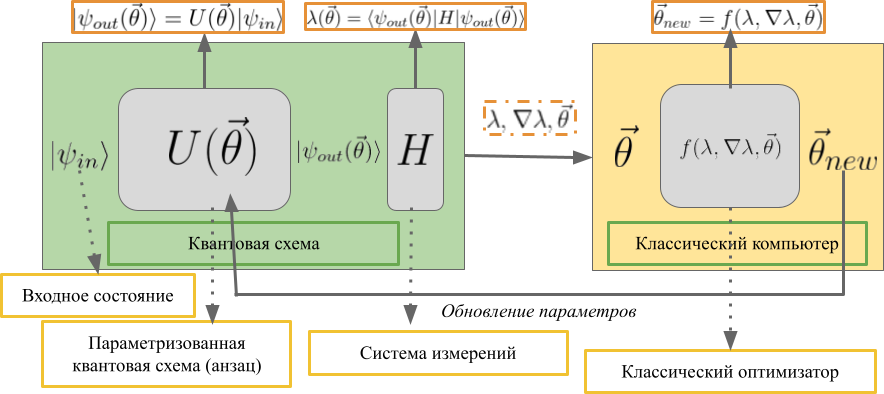
\includegraphics[scale=0.8]{VQA.png}}
\caption{блок-схема, иллюстрирующая принцип работы вариационных квантовых алгоритмов.}\label{fig:VQA}
\end{figure}

\qquad Поиск подходящих параметров анзаца проводится с использованием оптимизатора на классическом вычислительном устройстве. Решение оптимизационной задачи представляет из себя итеративный процесс обновления параметров анзаца в результате взаимодействия квантового устройства с классическим оптимизатором. Схематически процесс работы ВКА представлен на Рис.\ref{fig:VQA} и состоит из следующих этапов:

\qquad 0) \emph{Кодирование задачи в некоторую наблюдаемую квантового состояния}. Представление наблюдаемой в виде системы измерений над квантовым состоянием, реализуемой на квантовом устройстве (например, кодирование в строку матриц Паули):

\begin{equation}
 H=\sum_{i} c_{i} \hat h_{i} = \sum_{i} c_{i} \otimes^{N-1}_{j = 0} \hat \sigma^{j}_{*},
\end{equation} где $\hat h_{i}$ - наблюдаемые, отдельно измеряемые на квантовом устройстве, $c_{i}$ - коэффициенты в разложении наблюдаемой на строки Паули, $ \sigma_{*} \in \{\hat I,\hat \sigma_{X}, \hat \sigma_{Y}, \hat \sigma_{Z}  \} $, $\otimes^{N-1}_{j = 0} \hat \sigma^{j}_{*}$ - обозначение произвольной строки матриц Паули длины не более $N$.

\qquad 1) \emph{Инициализация параметров анзаца}:
Задаётся изначальный набор параметров анзаца, который фиксируют определённое состояние квантовых вентилей и тем самым задают определённое преобразование над входным состоянием. $\vec{\theta}^0 = \vec{\theta}_{init}$, где $\vec{\theta}^0$ параметры анзаца на 1-й итерации алгоритма, $\vec{\theta}_{init}$ - параметры инициализации.

\qquad Начало итерационного процесса повторяющегося фиксированное количество шагов или до достижения заданного критерия остановки):

\begin{equation}
i = 0; \psi(\vec{\theta}^{0}) = \psi(\vec{\theta}_{init}),
\end{equation} где $\psi$ - волновая функция квантовой системы.


\qquad 2) \emph{Приготовление состояния}. Входное состояние (обычно $|0 \rangle$) преобразуется анзацем в выходное состояние $|\psi_{i}\rangle$:


\begin{equation}
|\psi^{i}\rangle = |\psi (\vec{\theta}^{i})\rangle = U(\vec{\theta}^{i}) |0 \rangle,
\end{equation} где $\psi^{i}$ - волновая функция состояния на $i$-й итерации; $U(\vec{\theta}^{i})$ - преобразование, осуществляемое анзацем над входным состоянием.

\qquad 3) \emph{Измерение}. Выходное состояние поступает в фиксированную часть квантовой схемы, где производится измерения соответствующие заданной наблюдаемой согласно пункту 0. Данный процесс повторяется многократно для набора статистики измерений. Далее на основе статистики измерений оценивается выборочное математического ожидания наблюдаемой величины:

\begin{equation}
\lambda(\vec{\theta}^{i}) = \langle \psi(\vec{\theta}^{i}) |H|\psi(\vec{\theta}^{i})\rangle,
\end{equation} где $H$ - оператор наблюдаемой величины; $\lambda(\vec{\theta}^{i})$ - математическое ожидание наблюдаемой $H$, полученное на основе серии измерений выходного состояния.

\qquad Так же для большинства методов оптимизации необходимо произвести дополнительные измерения. Например, для градиентных методов требуется оценка $ \nabla_{\mathbf{\theta}^{i}} \lambda(\vec{\theta}^{i})$, которую можно получить с помощью правила варьирования параметров \cite{param_shift};
 
 \qquad 4) \emph{Расчет значения функции потерь для заданных параметров}. На данном этапе используя оценку выборочного среднего наблюдаемой и опционально другие квантовые и ли классические параметры составляется функция потерь $C$, минимизация которой соответствует решению рассматриваемой оптимизационной задачи. В роли опциональных квантовых параметров может выступать, например, степень перепутанности подсистем кубитов выходного состояния:

\begin{equation}
C = C(\lambda(\vec{\theta}^i), \vec{q}, \vec{c}),
\end{equation} где $\lambda(\vec{\theta}^i)$ - выборочное среднее наблюдаемой величины $H$ при параметрах анзаца $\vec{\theta}^i$, $q(\vec{\theta}^i)$ - опциональные квантовые параметры, $\vec{c}$ - опциональные классические параметры.

\qquad 5) \emph{Обновление параметров анзаца на классическом вычислительном устройстве}.
На данном этапе решается задача классической многомерной оптимизации, целью которой является минимизация заданной функции путём варьирования вектора её параметров. В зависимости от выбранного метода оптимизации меняется правило обновления параметров. В данной работе рассматривается градиентная оптимизация, для которой обновление параметров базовом виде выглядит следующим образом:

\begin{equation}
\vec{\theta}^{i+1} = \vec{\theta}^{i} - k \nabla_{\mathbf{\theta^{i}}} C(\vec{\theta}^{i}),
\end{equation} где $C(\vec{\theta}^{i})$ - функция потерь при заданных параметрах анзаца $\vec{\theta}^{i}$, $\vec{\theta}^{i}$ - параметры анзаца на $i$-й итерации, $k$ - коэффициент регулирующий величину шага оптимизации.


\qquad Заметим, что для дифференцируемой по параметрам функции потерь выражение для расчёта градиента $\nabla_{\mathbf{\theta}^{i}} C(\vec{\theta}^{i})$ можно раскрыть аналитически через частные производные выборочного среднего наблюдаемой $\frac{\delta C(\vec{\theta}^{i})}{\delta \theta^{i}_{j}} = \frac{\delta C}{\delta \lambda} \frac{\delta \lambda(\vec{\theta}^{i})}{\delta \theta^{i}_{j}}$, которые оценивается на квантовом устройстве. Это позволяет использовать частные производные,вычисленные на квантовом устройстве в классической оптимизации.


\qquad 6) \emph{Переход на новую итерацию или завершение оптимизационного процесса}. На данном этапе параметры вариационной схемы обновлены, запускается следующая итерация ВКА. Процесс длится заданное количество итераций, либо останавливается по достижению определённых условий.


\subsection[Применение вариационных квантовых алгоритмов]{Применение вариационных квантовых \linebreak алгоритмов}

\qquad ВКА являются потенциально перспективными алгоритмами для достижения квантового превосходства в проблемах физики многих тел, а так же оптимизационных комбинаторных задачах. Наиболее естественным способом использования ВКА является решение задач квантовой химии, таких как исследование статических и динамических свойств молекул и сильно корреллированных электронных систем, которые является фундаментальными задачами во многих областях науки. Например, такие задачи актуальны в биологии для понимания динамики сворачивания белков \cite{Outeiral_2020}, в фармацевтике для улучшения возможностей открытия лекарств \cite{10.1147/JRD.2018.2888987}, в производстве материалов для изучения высокотемпературной сверхпроводимости. В ядерной физике ВКА так же могут найти аналогичные применения для исследования энергетической структуры ядра частиц \cite{Dumitrescu_2018}. 


\qquad Второй потенциальной областью применения ВКА являются проблемы оптимизации. Основная предпосылка к применению ВКА для решения комбинаторных задач основана на возможности использования высокой размерности гильбертова пространства состояний квантовомеханической системы для кодирования оптимизационных проблем с надеждой на ускорение решения за счёт наличия квантовой запутанности кубитов ВКА. Одним из лидирующих кандидатов на достижение квантового превосходства среди ВКА благодаря особой структуре параметризованной части квантовой схемы, преобразование которой над входным состоянием не поддаётся классическому моделированию, признаётся КПОА \cite{https://doi.org/10.48550/arxiv.1411.4028}, предназначенный для решения комбинаторных задач.


\qquad Так же в отдельную область можно выделить применение ВКА в задачах машинного обучения. Наиболее перспективными алгоритмами в области квантового машинного обучения КМО (в англоязычной литературе quantum machine learning QML) на данный момент считаются квантовые нейронные сети КНН (в англоязычной литературе quantum neural netwoeks QNN). Для ряда задач показано, что КНН обучаются быстрее аналогичных классических нейронных сетей и требуют меньше оптимизируемых параметров для достижения заданного качества \cite{Abbas_2021}. Более того отдельный класс КНН свёрточные квантовые нейронные сети КСНН (в англоязачной литературе quantum convolution neural networks) не подвержены проблеме бесплодных плато \cite{QCNN}, типичной для ВКА, что открывает большие перспективы для их дальнейшего использования в задачах глубинного обучения, обработки изображений, обучения с подкреплением и тд.


\subsection{Основные трудности и пути решения}

\qquad Несмотря на возможные перспективы ВКА в эпоху шумных квантовых устройств средних размеров, их применение до сих пор связано с рядом проблем включая сложность оптимизируемости, точность результатов и эффективность применения ВКА в сравнении с классическими алгоритмами.

\qquad Наиболее серьёзной проблемой при минимизации функции потерь ВКА является наличие феномена, называемого бесплодным плато БП \cite{McClean_2018}. При использовании неструктурированных универсальных анзацев с увеличением размерности решаемой проблемы в среднем частные производные функции потерь экспоненциально быстро стремятся к нулю. Другими словами гиперповерхность параметров становится практически плоским и для поиска глобального минимума необходимо экспоненциально по размерности пространств долго оптимизироваться случайно блуждая по плоскому участку гиперповерхности, что делает использование ВКА неэффективным методом. Возникновение БП в универсальных анзацах можно считать следствием экспоненциального расширения гильбертова пространства оптимизации при увеличении количества перепутывающих вентилей в анзаце \cite{Holmes_2022}. Так же в серии работ было показано, что возникновение БП может быть вызвано высокой степенью запутанности системы кубитов, а так же наличием шума \cite{entangled_barren_plateaus}, \cite{noise_barren_plateaus}.

\qquad Так же для достижения квантового преимущества необходимо уметь эффективно проводить измерения с использованием ВКА. Нфпример, квантовой химии количество строк Паули в разложении гамильтонианов молекул растёт приблизительно как $~n^{4}$ с ростом количества орбиталей молекулы $n$. В работах \cite{Huggins_2021}, \cite{Yen_2021} предложены различные техники с использованием коммутирующих групп операторов измерения для возможности их одновременного измерения и как следствие сокращения общего числа необходимых измерений. 

\qquad Наличие шума в квантовых операциях является ещё одной проблемой использования ВКА. Воздействие шума приводит к ряду нежелательных последствий в виде возникновения БП даже в неглубоких схемах, а так же снижению точности результатов в сравнении с оптимизацией в отсутствии шума \cite{Wang_2021}.


\subsection{Система измерений и функция потерь}

\qquad Первым этапом в решении задачи оптимизации является кодирование минимизируемого функционала в физическую наблюдаемую и её представление в виде системы измерений над вектором состояния квантовой системы, приготавливаемым при помощи анзаца. В зависимости от поставленной задачи ВКА сводятся к алгоритмам ВКС или КПОА отличающимся различными способами кодирования минимизируемого значения наблюдаемой в систему измерений.

\qquad Для задач поиска определённых характеристик физической системы используется алгоритм ВКС, где в качестве минимизируемой величины выступает математическое ожидание анализируемой физической наблюдаемой для выходного состояния анзаца. Например, в задачах квантовой химии для поиска энергии основного состояния молекулы в роли наблюдаемой величины выступает её гамильтониан.

\qquad Наблюдаемая представляется в виде серии измерений в некотором базисе. Удобно в качестве базиса для однокубитовых измерений использовать матрицы Паули $ \{I,\sigma_{X}, \sigma_{Y}, \sigma_{Z}  \}$, тогда наблюдаемая может быть выражена в виде линейной комбинации строк матриц Паули:

\begin{equation}
\hat H=\sum_{i} c_{i} \hat h_{i} = \sum_{i} \hat c_{i} \otimes^{N-1}_{j = 0} \hat \sigma^{j}_{*},
\end{equation} где $ \sigma_{*} \in \{\hat I,\hat \sigma_{X}, \hat \sigma_{Y}, \hat \sigma_{Z}  \} $, $N$ - размерность системы кубитов.

\qquad Результатом измерений наблюдаемой выходного состояния является линейная комбинация математических ожиданий действия строк Паули на выходное состояние анзаца: 

\begin{equation}
\lambda(\vec{\theta}^{i}) = \langle \psi(\vec{\theta}^{i}) | \hat H | \psi(\vec{\theta}^{i}) \rangle = \langle \hat H \rangle =\sum_{i} c_{i} \langle \hat h_{i} \rangle = \sum_{i} \hat c_{i} \otimes^{N-1}_{j = 0} \hat \langle \sigma^{j}_{*} \rangle,
\end{equation} где $\psi(\vec{\theta}^{i})$ - вектор выходного состояния на $i$-й итерации; $ \sigma_{*} \in \{\hat I,\hat \sigma_{X}, \hat \sigma_{Y}, \hat \sigma_{Z}  \} $, $N$ - размерность системы кубитов.

\qquad Следующим шагом с использованием наблюдаемой составляется функция потерь, минимум которой совпадает с решением задачи. В простейшем случае функция равняется математическому ожиданию наблюдаемой:

\begin{equation}
 C(\lambda(\vec{\theta}^i)) = \lambda(\vec{\theta}^i),
\end{equation}  где $\lambda(\vec{\theta}^i)$ - выборочное среднее наблюдаемой величины.

\qquad В общем случае функция потерь зависит не только от оценки математического ожидания наблюдаемой величины на квантовом устройстве. В аргументы могут входить и другие опциональные величины, которые возможно оценить на квантовом устройстве. Так же аргументами функции потерь могут являться и чисто классические параметры:

\begin{equation}
C = C(\lambda(\vec{\theta}^i), \vec{q}, \vec{c}),
\end{equation} где $\lambda(\vec{\theta}^i)$ - выборочное среднее наблюдаемой величины $H$ при параметрах анзаца $\vec{\theta}^i$, $q(\vec{\theta}^i)$ - опциональные квантовые параметры, $\vec{c}$ - опциональные классические параметры.

\qquad В некоторых специфических областях применения ВКА, таких как квантовая коррекция ошибок, квантовая метрология, вариационное решение линейных уравнений и тд., функция потерь может быть представлена принципиально другим образом. Более того в некоторых случаях представляется возможность задать локальную функцию потерь, вместо глобальной ( оцениваются только однокубитовые наблюдаемые и потом суммируются, в отличие от глобальной функции потерь, где оценивается наблюдаемая, действующая на полное состояние квантовой системы). Доказано, что локальные функции потерь меньше подвержены возникновению БП и соответственно значительно более эффективны в использовании \cite{Cost_func_and_landscape}.

\subsection{Анзац}

\qquad Анзац ВКА, как отмечалось выше, представляет из себя параметризованную квантовую схему, которая готовит различные в зависимости от параметризации состояния системы. Анзац применяется для поиска квантового состояния, минимизирующего значение наблюдаемой. 

\begin{figure}[H]
\center{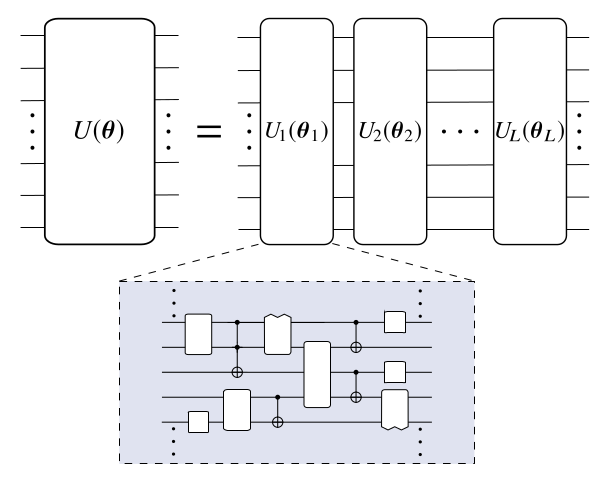
\includegraphics[scale=0.5]{layers_anzatz.png}}
\caption{Иллюстрация, демонстрирующая представление анзаца параметризованной квантовой схемы в виде слоистой структуры.}\label{fig:layers_anzatz}
\end{figure}

\qquad В общем случае анзац может быть представлен в виде слоистой структуры (см. рис. \ref{fig:layers_anzatz}), тогда преобразование над входным состоянием можно записать в виде произведения:

\begin{equation}
U(\vec \theta) = U_{L}(\vec{\theta}_{L}) \cdots U_{2}(\vec{\theta}_{2}) U_{1}(\vec{\theta}_{1}),
\end{equation} где 

\begin{equation}
U_{l}(\vec{\theta}_{l}) = \prod_{m} e^{-i \theta_{m} H_{m} } W_{m},
\end{equation} где $W_{m}$ - непараметрическое унитарное преобразование, а $H_{m}$ - эрмитов оператор.


\qquad Выбор анзаца чрезвычайно важен для эффективной работы ВКА, так как именно анзац задаёт пространство возможных преобразований над состоянием квантовой системы и как результат пространство выходных состояний. В основном для описания анзаца используются такие его характеристики, как выразительность (в англоязычной литературе называемая "expressibility") и средняя мера запутанности выходных состояний \cite{Sim_2019}.


\qquad Выразительность анзаца является мерой сходства пространства преобразований, которые можно получить варьирую его параметры и пространства всевозможных состояний заданной размерности. Таким образом максимально выразительный анзац со случайно заданными из равномерного распределения параметрами с равной вероятностью совершает произвольное унитарное преобразование над квантовым состоянием. Для количественной оценки выразительности анзаца используется сравнение распределения состояний полученных на выходе случайно инициализированного анзаца $U(\vec \theta)$ с максимально выразительным распределением квантовых состояний, распределением Хаара. Описанная мера выразительности называется мерой Хаара \cite{_yczkowski_2005} и для $t$ - го момента описывается формулой:

\begin{equation}
A^{(t)}(U) = \int dU_{Haar}U^{\otimes t}_{Haar} |0 \rangle |0 \langle 0 | {(U^{\dagger}_{Haar})}^{\otimes t} - \int dU U^{\otimes t} |0 \rangle |0 \langle 0 | {(U^{\dagger})}^{\otimes t},
\end{equation} где $U_{Haar}$ - преобразование готовящее равномерно распределённые по Хаару состояния, $U$- унитарное преобразование анзаца.

\qquad Возможность использования выбранного анзаца для решения задачи обусловлена достаточной выразительностью анзаца для приготовления, состояние соответствующего решению задачи. При этом высокая выразительность анзаца обычно негативно сказывается на процессе оптимизации, так как значительно усложняет поиск глобального минимума функции потерь. В частности высокая выразительность анзаца связана с появлением БП, так как гильбертовом пространств оптимизации  экспоненциально растёт с увеличением размерности системы.

\qquad Так же было показано, что помимо большой выразительности анзаца причиной появления БП может стать высокая запутанность состояния приготавливаемого анзацем. Таким образом анзацы с высокой средней запутанностью выходного состояния с большой вероятностью подвержены возникновению БП.

\qquad Существует два основных подхода к реализации анзаца. Первый называется аппаратно-эффективным и заключается в использовании универсального анзаца, элементы и архитектура которого легко реализуется на выбранном квантовом устройстве. Такой подход перспективен в первую очередь ввиду его универсальности для произвольной проблемы и простоты реализации. Особенно эффективно применение к гамильтонианам схожей структуры с архитектурой анзаца. При этом аппаратно-эффективный универсальный анзац приводит к сложностям в оптимизации и возникновению БП в связи с высокой выразительностью анзаца. В ряде случаев данную проблему помогает избежать эффективная инициализация начальных параметров.

\qquad Второй подход основан на идее использования информации о решаемой проблеме для построения архитектуры анзаца, получая в результате "вдохновлённую проблемой"\ архитектуру анзаца. Такой подход позволяет сильно понизить выразительность анзаца, значительно ускоряя процесс оптимизации, и снижая вероятность появления БП, при этом гарантируя достижимость состояния минимизирующего наблюдаемую.

\subsection{Инициализация параметров} 

\qquad Процесс оптимизации параметризованной схемы ВКА начинается с инициализации параметров. Случайная инициализация параметров, особенно в универсальных анзацах, зачастую приводит к застревании процесса оптимизации на БП. При этом правильно выбранные начальные параметры могут помочь оптимизатору не попасть в БП, когда оно присутствует на гиперповерхности функции потерь.

\qquad В литературе рассматривается множество подходов к эффективной инициализации начальных параметров. Например, в работе \cite{Skolik_2021} предлагается оптимизировать анзац слой за слоем, чтобы при добавлении нового слоя с большой вероятностью вектор параметров соответствовал точке в пространстве оптимизации, близкой к глобальному минимуму частичного анзаца, что позволяет оптимизатору избежать БП и достигнуть глобального минимума полного анзаца. В работе \cite{Grant_2019} предлагается разбить слоистый анзац на $D$ блоков по $2K$ слоёв и инициализировать в каждом блоке первые $K$ слоёв случайно, а последующие так чтобы каждый блок в результате давал единичное преобразование:

\begin{multline}
U(\vec \theta) = [U_{L}(\vec{\theta}_{L}) \cdots U_{L-K}(\vec \theta_{L-K}) U^{\dagger}_{L-K-1}(\vec \theta_{L-K-1} U^{\dagger}_{L-2K}(\vec \theta_{L-2K})]  \cdots \\ 
[U_{2K}(\vec \theta_{2K}) \cdots U_{K}(\vec \theta_{K}) U^{\dagger}_{K-1}(\vec \theta_{K-1} U^{\dagger}_{0}(\vec \theta_{0})] =  \\  U^{*}_{D}(\vec  \theta_{L} \cdots \vec  \theta_{L-2K}) \cdots U^{*}_{0}(\vec \theta_{2K} \cdots \vec  \theta_{0}) =  I_{D} \cdots I_{0} = I,
\end{multline}

где $U_{l}(\vec \theta_{l})$ - преобразование $l$-го слоя анзца над входным состоянием при заданных параметрах  $l$-го слоя $\vec \theta_{l}$; $U^{*}_{d}(\vec  \theta_{l} \cdots \vec  \theta_{l-2k}) $ - преобразование $d$-го блока из $2k$ слоев анзаца над входным состоянием; $I_{d}$ - единичное преобразование, соответствующее $d$-му блоку анзаца.

\qquad Инициализация единичными блоками даёт возможность рассматривать анзац на первых шагах, как неглубокий и с малой степенью запутанности, гарантируя инициализацию начальных параметров на некотором отдалении от БП. 

\subsection{Классический оптимизатор}

\qquad Классический оптимизатор итеративно обновляет параметры анзаца для достижения минимального значения функции потерь $ C = C(\lambda(\vec \theta^{i}), ...)$, зависящей от оценки математического ожидания наблюдаемой при заданных параметрах $\vec \theta$  и дополнительных.  Таким образом задача оптимизатора формулируется в виде  $min_{\vec \theta} ( \langle \psi(\vec{\theta^{i}}) |C|\psi(\vec{\theta}^{i})\rangle )$. На каждой итерации на вход оптимизатор принимает вектор параметров $\vec \theta^{i} $, значение функции потерь при заданном векторе  параметров $С(\vec \theta^{i}) $, а так же дополнительные характеристики в зависимости от метода,далее вычисляется обновлённый вектор параметров $\vec \theta^{i+1} $ и передаётся на квантовое устройство для перехода на следующую итерацию.

\qquad Оптимизаторы делятся на градиентные и безградиентные по принципу обновления параметров. Оптимизационные методы не использующие градиент в основном являются эвристическими. Такие методы оптимизации основаны на естественных процессах, приводящих к оптимальным результатам. К безградиентным методам относятся генетические алгоритмы, алгоритм роя частиц, алгоритм симуляции отжига.


\qquad Градиентные методы используют принципиально другой подход к оптимизации. Итеративное обновление параметров в общем виде происходит по методу градиентного спуска согласно следующей формуле:

\begin{equation}
\vec{\theta}^{i+1} = \vec{\theta}^{i} - k \nabla_{\mathbf{\theta^{i}}} C(\lambda (\vec \theta^{i})),
\end{equation} где $\vec{\theta}^{i}$ - параметры анзаца с предыдущей итерации, $\vec{\theta}^{i+1}$ - обновлённые параметры анзаца $C(\lambda (\vec \theta^{i}))$ - минимизируемая функция потерь.
 

\qquad Заметим, что градиент функции потерь рассчитывается также на квантовом устройстве. Стандартным способом расчёта частной производной функции потерь на квантовом устройстве является правило варьирования параметра (в англоязычной литературе называемый parameter shift rule):

\begin{equation}
 \frac{\partial  \lambda (\vec \theta)}{\partial \theta_{i}} = \frac{ \lambda (\theta_{0},..., \theta_{i} + \frac{\pi}{2}, ..., \theta_{K}) - \lambda (\theta_{0},..., \theta_{i} - \frac{\pi}{2}, ..., \theta_{K})}{2},
\end{equation} где $\lambda(\vec \theta)$ - математическое ожидание наблюдаемой величины при заданных параметрах анзаца, $\theta_{i}$ - i-й элемент вектора параметров $\vec \theta$.

\qquad Оценка градиента рассчитывается с использованием правила варьирования параметров за $2T$ запусков, где $T$ - размерность вектора параметров $\vec \theta$. 

\qquad Существует множество модификаций градиентного спуска, увеличивающих скорость сходимости и точность результата, способствуя выходу из локальных минимумов. Одним из наиболее популярных оптимизаторов в классическом машинном обучении, где также необходимо решать задачи оптимизации высокой размерности, является метод адаптивной оценки моментов АдаМ \cite{https://doi.org/10.48550/arxiv.1412.6980} (в англоязычной литераторе adaptive moment estimation AdaM). Данный алгоритм способствует выходу из локальных минимумов за счёт наличия инерции в оценке градиента на новой итерации, а так же учитывает важность оптимизации по каждому из параметров, оценивая накопительную дисперсию. Алгоритм обновления параметров методом АдаМ выглядит следующим образом:

\begin{equation}
\vec{\theta}^{(t+1)} = \vec{\theta}^{(t)} - \eta^{(t+1)} \frac{a^{(t+1)} }{   \sqrt{b^{(t+1)}} + \epsilon},
\end{equation} где $a^{(t+1)}$ накопительная оценка градиента на $t+1$ итерации, $b^{(t+1)}$ накопительная оценка нецентрированной дисперсии на $t+1$ шаге, $\eta^{(t+1)}$ - нормировочный коэффициент на $t+1$ шаге, $\vec \theta$ - варьируемый вектор параметров.

\qquad Существуют так же градиентные методы, требующие дополнительной информации о функции потерь. На данный момент одним из ведущих таких методов, который возможно реализовать на гибридном устройстве является квантовый натуральный градиент КНГ \cite{Stokes_2020} (в англоязычной литературе quantum natural gradient QNG). Обыкновенный градиентный спуск на каждом шаге использует градиент функции потерь в евклидовом пространстве, но в случае ВКА пространство оптимизации не является Евклидовым. КНГ учитывает неевклидовость пространства оптимизации с помощью умножения градиента функции на метрический тензор Фубини-Штуди который оценивается на квантовом устройстве каждом шаге $t$ - му шагу.


\begin{equation}
\vec{\theta}^{(t+1)} = \vec{\theta}^{(t)} - \eta g ( С( \vec{\theta}^{(t)} )  )^{-1} \nabla С( \vec{\theta}^{(t)}  ),
\end{equation} где $g ( C( \vec{\theta}^{(t+1)} )  )$ - метрический тензор функции потерь в точке соответствующей вектору параметров на $t$ шаге.

\qquad Оценка метрического тензора проводится на квантовом устройстве согласно следующему выражению:

\begin{equation}
g_{ij}^{(l)} = \langle \psi_{l} | K_{i}K_{j} |\psi_{l}  \rangle - \langle \psi_{l} | K_{i} | \rangle  \langle \psi_{l} | K_{j} |\psi_{l}  \rangle ,
\end{equation} где $K^{(l)}_{i}$ - генератор $i$-го квантового вентиля на $l$-м слое анзаца; $|\psi_{l}  \rangle$ - выходное состояние после $l$-го слоя анзаца.

\qquad Таким образом реализация КНГ на квантовом устройстве с оценкой градиента с помощью правила варьирования параметра для анзаца с $L$ слоями и $T$ параметрами требуется провести $E = 2T + L$ оценок на каждом шаге оптимизации. Заметим, что для неглубоких анзацев большой размерности $L<<T$, следовательно количеств дополнительных необходимых измерений незначительно в сравнении со стандартным градиентным спуском ($2T + L ~ 2T$).

\subsection[Применение вариационных квантовых алгоритмов к задачам квантовой химии]{Применение вариационных квантовых \linebreak алгоритмов к задачам квантовой химии}

\qquad Множество задач квантовой химии может быть решено с применением ВКС. В частности, ВКС можно использовать для поиска энергетического спектра, дипольного момента и других характеристик заданной молекулы. Наиболее простой задачей из перечисленных является поиск энергии основного состояния молекулы. 

\qquad Для поиска энергии основного состояния заданной молекулы с помощью ВКС для начала нужно представить гамильтониан молекулы в виде линейной комбинации строк матриц Паули. Это можно осуществить с помощью преобразований Джордана-Вигнера \cite{article}, Брави-Китаева \cite{Seeley_2012} или преобразования чётности (в англоязычной литературе Parity transform \cite{https://doi.org/10.48550/arxiv.hep-th/9312092}). Описанные преобразования имеют свои преимущества, например, преобразование чётности позволяет учесть симметрию молекулы, если она имеется, и за счёт этого эффективнее представить гамильтониан молекулы в виде строк матриц Паули. В данной работе изучаются свойства анзаца, и не поднимается вопрос эффективности представления молекулы в виде строк Паули, поэтому используется наиболее простое из перечисленных преобразование Джордана-Вигнера.

\qquad Система $N$ фермионов может быть описана при помощи детерминанта Слэтера, который представляет из себя антисимметричную относительно перестановки частиц волновую функция многочастичной квантовомеханической системы, построенную из одночастичных функций:



\begin{equation}
\Psi{(x_1, ... , x_N)} = \frac{1}{\sqrt{N!}} det \left(
\begin{array}{cccc}
\psi_{1} (x_1) & \psi_{1} (x_2) & \ldots & \psi_{1} (x_N)\\
\psi_{2} (x_1) & \psi_{2} (x_2) & \ldots & \psi_{2} (x_N)\\
\vdots & \vdots & \ddots & \vdots\\
\psi_{N} (x_1) & \psi_{N} (x_2) & \ldots & \psi_{N} (x_N)
\end{array}
\right),
\end{equation} где $\psi_{n} (x)$ - одночастичная волновая функция $n$-й частица системы, а $x_n$ - её координата.

\qquad Далее можно ввести некоторый базис $\{ \lambda_n \}^{N}_{n = 1}$ из $N$ состояний и представить многочастичную волновую функцию через числа заполнения:

\begin{equation}
|n_1,  \ldots  , n_{\lambda} \rangle = |(\lambda_1)_{n_1 \ раз} \leq \lambda_2)_{n_2 \ раз} \leq  \ldots  \leq (\lambda_N)_{n_N \ раз} \rangle,
\end{equation} где числа заполнения для фермионов согласно принципу Паули $n_{\lambda} \in \{ 0,1 \}$.


\qquad Далее можно перейти к описанию через набор операторов рождения $\{ a_{p} \}^{N-1}_{p=0} $ и уничтожения $\{ a^{\dagger}_{p} \}^{N-1}_{p=0} $, которые удовлетворяют антикоммутационным соотношениям:

\begin{eqnarray}
	\{ a_{p}, a_{q} \} = 0, \
	\{ a_{p}, a^{\dagger}_{q} \} = \delta_{pq},
\end{eqnarray} где $a_{p}$ - оператор уничтожения, действующий на p-ю моду/

\qquad Тогда действие операторов рождения и уничтожения на систему фермионов представляется в виде:

\begin{equation*}
a_p | n_0, \ldots, n_{p-1}, 1, n_{p+1}, \ldots, n_{N-1} \rangle = ...
\end{equation*}
\begin{equation}
 = (-1)^{\sum^{p-1}_{q=0} n_q} | n_0, \ldots, n_{p-1}, 1, n_{p+1}, \ldots, n_{N-1} \rangle
\end{equation}
\begin{equation*}
a_p | n_0, \ldots, n_{p-1}, 1, n_{p+1}, \ldots, n_{N-1} \rangle = 0,
\end{equation*} где $ n_p $ - числа заполнения в $n$-й моде.

\qquad В описанном формализме преобразования Джордана-Вигнера из фермионных операторов в кубитовые представляются в виде:

\begin{equation}
a_p \rightarrow \frac{1}{2}(X_{p} + iY_p)Z_1 \ldots Z_{p-1} = (| 0 \rangle \langle 1 |)_p Z_1 \ldots Z_{p-1}
\end{equation}, где $X_i, Y_i, Z_i$ - матрицы Паули, действующие на моду $i$.

\qquad При этом описывать точное взаимодействие всей системы множества тел чрезвычайно трудоёмко и разумно использовать аппроксимацию волновой функции заданной системы множества тел. Такую аппроксимацию можно получить пользуясь Пост-Хартри-Фоковскими методами электронной корреляции, \cite{Shikano_2021} которые представляют волновую функцию многих тел как линейную комбинацию детерминант Слейтера, обычно называемых конфигурациями. Эти конфигурации генерируются возбуждением электронов с занятых на незанятые HF-орбитали. Поскольку количество конфигураций комбинаторно увеличивается с количеством электронов и орбиталей можно ограничить степени свободы, определив активное пространство.

\begin{figure}[H]
\center{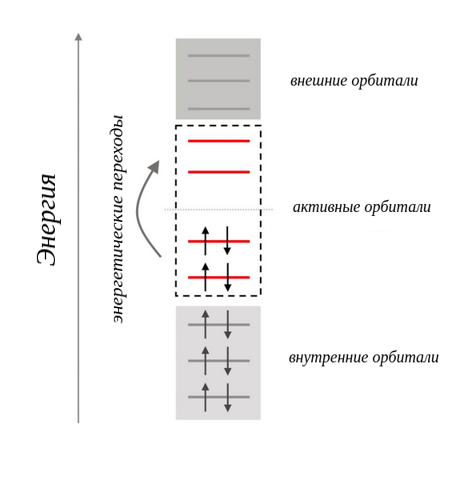
\includegraphics[scale=0.5]{active_orbitals.png}}
\caption{Иллюстрация демонстрирует выделение активных орбиталей и электронов в энергетическом спектре.} \label{fig:active_orbitals}
\end{figure}

\qquad Определение активного пространства происходит посредством выделения неактивных всегда занятых 2-мя электронами внутренних орбиталей и всегда свободных внешних орбиталей и ограниченного количества промежуточных активных орбиталей, населённость которых может варьироваться (см. рис.\ref{fig:active_orbitals} ).


\newpage

\begin{center}
\section[ТЕХНИЧЕСКАЯ РЕАЛИЗАЦИЯ ВАРИАЦИОННЫХ КВАНТОВЫХ АЛГОРИТМОВ]{ТЕХНИЧЕСКАЯ РЕАЛИЗАЦИЯ \linebreak ВАРИАЦИОННЫХ КВАНТОВЫХ \linebreak АЛГОРИТМОВ} \label{sec:technical_realization_section}
\end{center}


\subsection{Основные понятия}

\qquad В данном параграфе рассматривается физическая реализация анзаца и системы измерений кодирующей наблюдаемую. Для физической реализации могут быть выбраны квантовые устройства, основанные на различных технологиях (оптические интегральные схемы, атомы в ловушках, сверхпроводящие цепи или квантовые точки). При этом для любой выбранной технологии необходимо эффективно использовать физические ресурсы для реализации желаемой логической схемы.

\begin{figure}[H]
\center{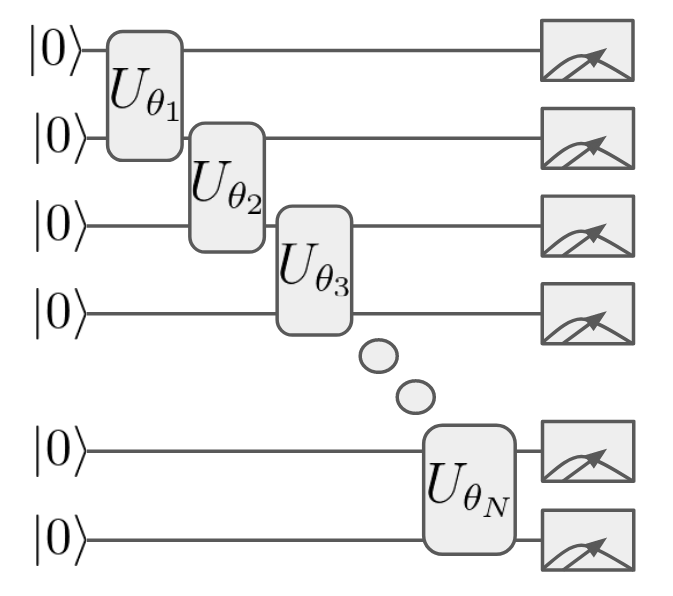
\includegraphics[scale=0.4]{MPS.png}}
\caption{Иллюстрация демонстрирует логическую схему однослойного анзаца с повторным использованием двухкубитового блока.}\label{fig:MPS}
\end{figure}

\qquad Существует отдельный класс цепочных анзацев для эффективного приготовления состояний матричного произведения МПС (в англоязычной литературе matrix product state MPS).  МПС может в точности моделировать только системы с одномерной геометрией, при этом подходит и для грубого описания систем с более сложными связями. МПС можно приготовить используя диагональный анзац \ref{fig:MPS}.

\begin{figure}[H]
\center{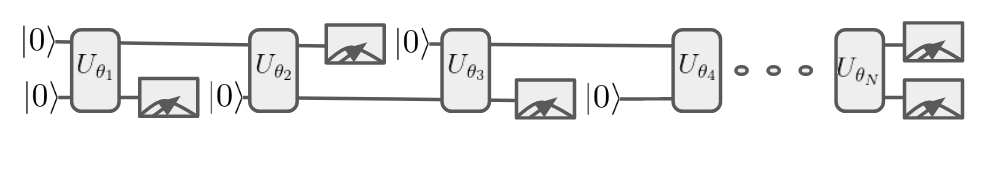
\includegraphics[scale=0.45]{MPS2.png}}
\caption{Иллюстрация демонстрирует эффективную физическую реализацию однослойного диагонального анзаца с повторным использованием двухкубитового перепутывающего блока.}\label{fig:MPS2}
\end{figure}

\qquad Заметим, что однослойный анзац с рис.\ref{fig:MPS} физически можно реализовать, повторно используя каналы логического блока в виде \ref{fig:MPS2}:

\qquad МПС малой размерности эффективно моделируется классически \cite{PhysRevLett.91.147902}, но при этом благодаря возможности повторно использовать физические кубиты на квантовом устройстве возможно создать МПС состояния размерности, недоступной для классического моделирования \cite{Liu_2019}.

\qquad Несмотря на одномерную геометрию МПС однослойные диагональные анзацы являются универсальными и были успешно применены к системам с различной геометрией связей \cite{doi:10.1146/annurev-conmatphys-020911-125018}. Успех применения МПС заключаются в том, что многие представляющие интерес физические и химические системы демонстрируют относительно малую запутанности в основных состояниях \cite{RevModPhys.82.277}.

\qquad Не всегда удается достигнуть основного состояния рассматриваемого гамильтониана, используя однослойный анзац, так как для систем большой размерности он способен приготовить лишь узкий класс состояний, в который может не попасть искомое основное состояние. В таких случаях можно рассмотреть более сложные архитектуры анзацев эффективно повторно использующие кубиты. В работе \cite{universal_linear_loop} представлен алгоритм использования зацикленных оптических схем для эффективной реализации слоистых анзацев вида:


\begin{figure}[H]
\center{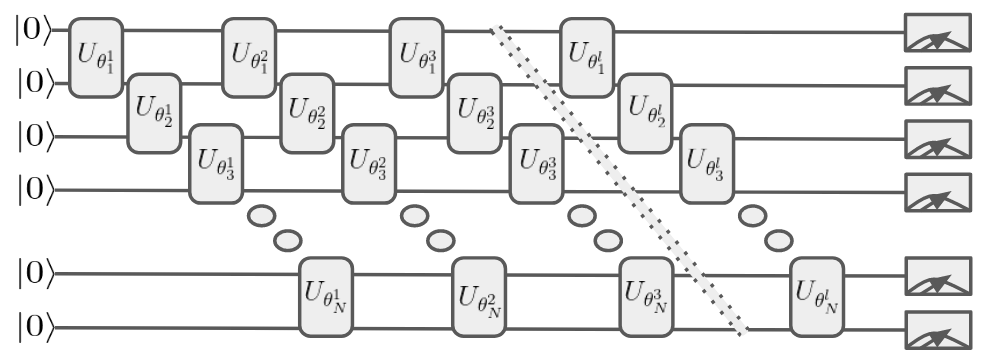
\includegraphics[scale=0.45]{layered_ansatz.png}}
\caption{Иллюстрация демонстрирует логическую схему многослойного диагонального анзаца.}\label{fig:layered_ansatz}
\end{figure}

\qquad Авторы данной работы рассматривают цепочные зацикленные схемы, а так же схемы с двойным циклом, представленные на рис. \ref{fig:loop_architectures} для приготовления крупномасштабных оптических схем с использованием компактных устройств с малым количеством оптических элементов за счёт повторного использования ресурсов. 



\begin{figure}[H]
\begin{center}
\begin{minipage}[h]{0.79\linewidth}
\center{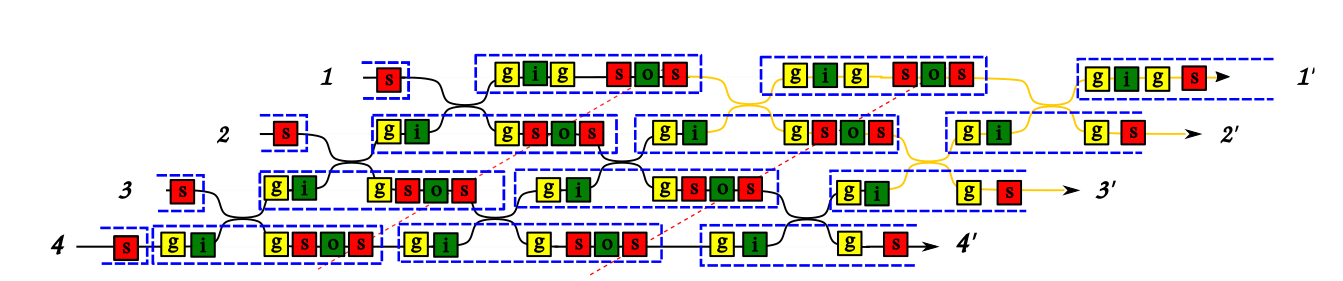
\includegraphics[width=\textwidth]{dual_loop_ansatz.png} а)}
\end{minipage}
\vfill
\begin{minipage}[h]{0.79\linewidth}
\center{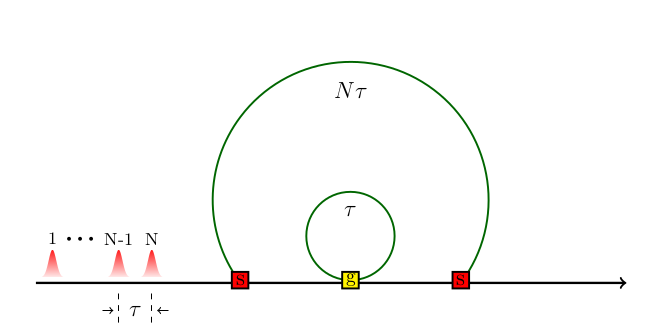
\includegraphics[width=\textwidth]{dual_loop.png} б)}
\end{minipage}
\vfill
\begin{minipage}[h]{0.79\linewidth}
\center{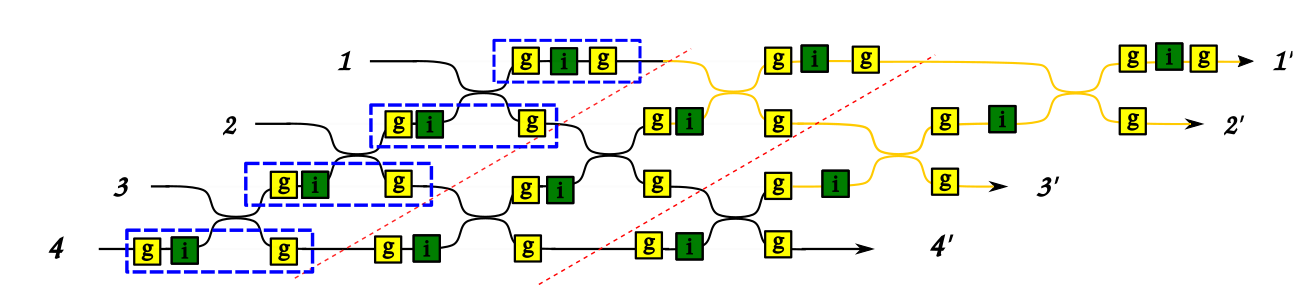
\includegraphics[width=\textwidth]{chain_loop_ansatz.png} в)}
\end{minipage}
\vfill
\begin{minipage}[h]{0.79\textwidth}
\center{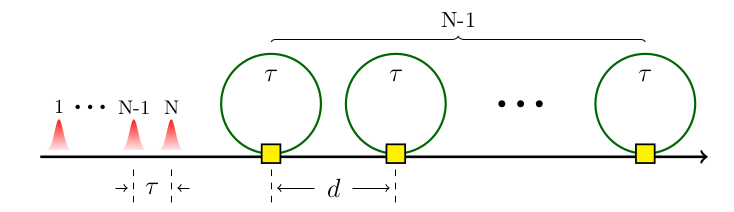
\includegraphics[width=\textwidth]{chain_loop.png} г)}
\end{minipage}
\end{center}
\caption{ Иллюстрация демонстрирует общий вид крупных линейно-оптических схем, полученных на основе повторного использования интерферометров малой размерности при помощи: а) зацикленной схемы с двойным циклом; в) зацикленной схемы цепочного вида, и соответствующие им физические реализации б),г). Блоки $"i"$ и $"o"$ зелёного цвета, соответствуют использованию внутренней и внешней петли задержки (внешняя петля имеется только в схеме с двойным циклом), блоки $"g"$ жёлтого цвета соответствуют быстрым управляемым интерферометрам Маха-Цендера, а блоки $"s"$ красного цвета быстрым управляемым переключателем между каналами \cite{universal_linear_loop} .}\label{fig:loop_architectures}
\end{figure}


\qquad Оптическая схема с двойным циклом позволяет построить слоистые диагональные анзацы (рис. \ref{fig:layered_ansatz}) используя всего один физический двухканальный блок и две петли зацикливания, отношение задержек в которых равно размерности рассматриваемой системы. Основным минусом такой схемы являются высокие потери реализации внешней петли зацикливания, которые экспоненциально возрастают по отношению к размерности системы. Цепочная петлевая схема является компромиссом между пространственной сложностью реализации и накапливаемой в процессе зацикливания ошибкой. Для реализации такой архитектуры требуется $l$ двухкубитовых блоков, где $l$ - число слоёв в анзаце, при этом пропадает внешнее кольцо зацикливания и сокращаются ошибки.

\qquad Другой способ использования зацикленных схем для повторного использования кубитов, получивший название галографического МПС, рассматривается в работе \cite{Foss_Feig_2021}. Авторы предлагают делить схему на более крупные блоки для их дальнейшего повторного использования, как это продемонстрировано на рис. \ref{fig:MPS_compl}. Главным преимуществом такого подхода является возможность реализации на любом типе квантовых устройств и широкий выбор геометрии квантовой схемы без потери качества. При этом количество физически используемых двухкубитовых блоков растёт полиномиально относительно количества слоёв анзаца.

\begin{figure}[H]
\center{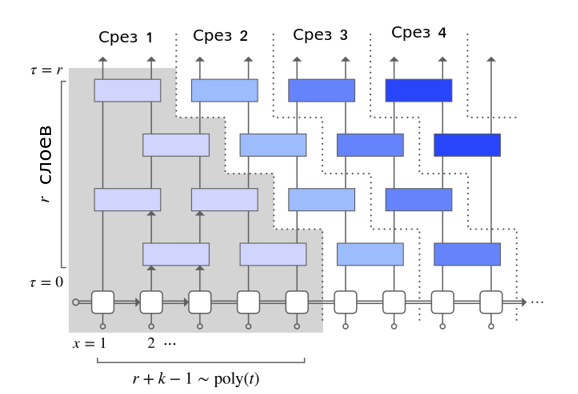
\includegraphics[scale=0.6]{MPS_compl.png}}
\caption{Блок-схема, иллюстрирует принцип галографического метода построения анзаца большой размерности при помощи повторного использования физической схемы малой размерности. На схеме блоки обозначают некоторое двухкубитовые параметризованные преобразования. В каждый момент времени физически реализован только один срез рассмотренной логической схемы \cite{Foss_Feig_2021} .}\label{fig:MPS_compl}
\end{figure}


\qquad В данной работе рассматривается обобщение многослойного диагонального анзаца, дополненного блоками перестановок кубитов между слоями (см рис. \ref{fig:layered_ansatz_permut}). Такое преобразование позволяет рассматривать схемы с произвольным порядком двухкубитовых гейтов, для реализации более эффективных архитектур при тех же затратах, например полностью запутанный слой (в англоязычной литературе strongly entengled layer), где имеются двухкубитовые операции между каждой парой кубитов. 


\begin{figure}[H]
\begin{minipage}[h]{0.81\linewidth}
\center{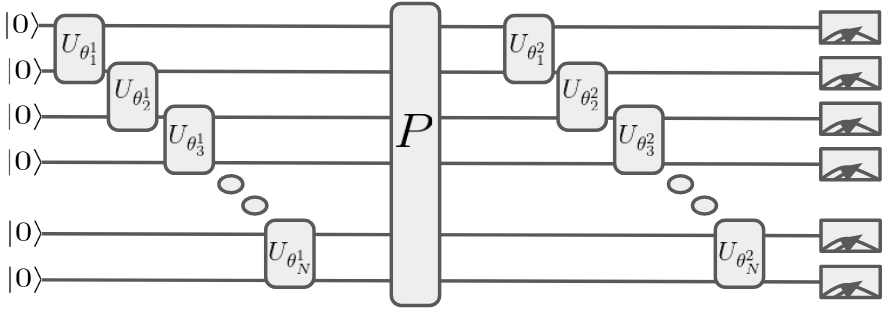
\includegraphics[width=\textwidth]{layered_ansatz_permut.png} а)}
\end{minipage}
\hfill
\begin{minipage}[h]{0.18\linewidth}
\center{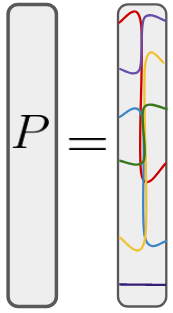
\includegraphics[width=\textwidth]{permutation.png} б)}
\end{minipage}
\vfill
\begin{minipage}[h]{1.\linewidth}
\center{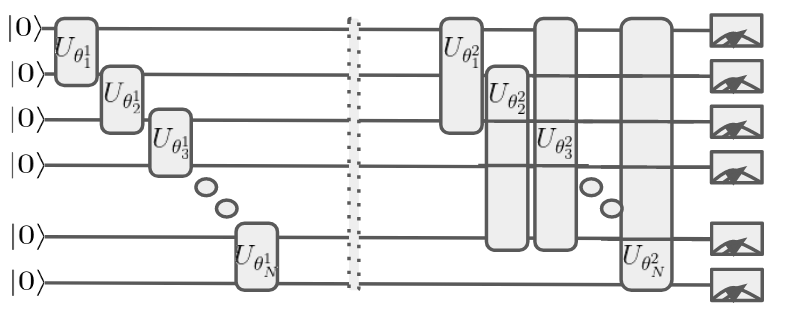
\includegraphics[width=\textwidth]{layered_ansatz_permut2.png} в)}
\end{minipage}
\caption{Блок-схема, иллюстрирует логическую схему обобщения слоистого диагонального анзаца с добавлением перестановочных блоков между кубитами: а) схематическое изображение обобщённого слоистого диагонального анзаца; б) схематическое изображение принципа работы перестановочного блока; в) схематическое изображение обобщённого слоистого анзаца, представленное в явном виде после действия перестановочных блоков.}\label{fig:layered_ansatz_permut}
\end{figure}

\qquad Обобщение слоистого анзаца может быть реализовано по аналогии с диагональным слоистым анзацем при помощи добавления программируемой линии задержки между слоями.


\subsection{Перепутывающий блок анзаца}

\qquad В качестве двухкубитового перепутывающего блока в схеме могут быть использованы преобразования произвольного вида.

\begin{figure}[H]
\begin{minipage}[H]{0.54\linewidth}
\center{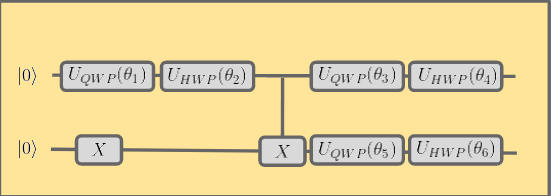
\includegraphics[width=\textwidth]{uni_ansatz.png} а)}
\end{minipage}
\hfill
\begin{minipage}[H]{0.44\linewidth}
\center{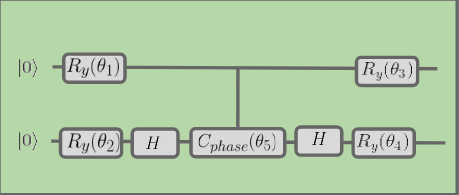
\includegraphics[width=\textwidth]{Cphase_ansatz.png} в)}
\end{minipage}
\vfill
\begin{minipage}[H]{0.37\linewidth}
\center{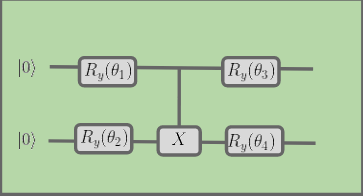
\includegraphics[width=\textwidth]{Cnot_ansatz.png} б)}
\end{minipage}
\hfill
\begin{minipage}[H]{0.62\linewidth}
\center{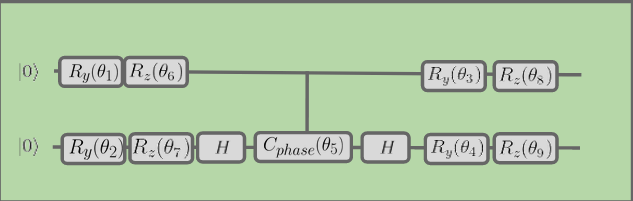
\includegraphics[width=\textwidth]{Cphase_HEA_RZ_ansatz.png} г)}
\end{minipage}
\caption{Блок-схема, иллюстрирует логические схемы сравниваемых двухкубитовых блоков анзаца. a) Универсальный двухкубитовый перепутывающий блок $B_{uni}$, способный приготовить произвольное двухкубитовой состояние. Блоки $U_{HWP}$ и $U_{QWP}$ добавлены для краткости записи и обозначают соответствующие логические элементы, а не физические пластины; б) $B_{RY}$ перепутывающий блок, использующий в качестве однокубитовых преобразований только $RY(\vec \theta)$; в) $B_{Cphase.RY}$ двухкубитовый перепутывающий блок; г) $B_{RZ.RY}$ двухкубитовый перепутывающий блок.}\label{fig:block_comp}
\end{figure}

\qquad В данной работе сравниваются 4 вида двухкубитовых перепутывающих блока (см. рис. \ref{fig:block_comp}). Рассматривается (а) универсальный двухкубитовый блок (далее именуется $B_{uni}$), способный осуществить произвольное преобразование над  входным состоянием, (б) блок, использующий в качестве однокубитовых операций только $RY(\vec \theta)$ вентили, преимущества которого описаны в \cite{https://doi.org/10.48550/arxiv.1909.05074}, (далее именуется $B_{RY}$ перепутывающий блок), (в) модернизация $B_{RY}$ блока с добавлением контроля максимальной запутанности с заменой вентиля $CNOT$ на $HCphase(\vec \theta)H$ (далее именуется $B_{Cphase RY}$ перепутывающий блок) и (г) модернизация $B_{RY}$ перепутывающего блока с добавлением дополнительных $RZ(\vec \theta)$ вентилей (далее именуется $B_{RZ RY}$ перепутывающий вентиль).


\qquad Использование универсального двухкубитового блока $B_{uni}$  позволяет приготовление произвольное двухкубитовое состояние, при этом анзац характеризуется выской выразительностью, и соответственно высокой вероятность попасть на БП в процессе оптимизации не дойдя до искомого минимального значения функции потерь. $B_{RY}$ двухкубитовый перепутывающий  блок, в свою очередь не является универсальным, так как характеризуется всего 4-мя параметрами, но при этом значительно меньше подвержен проблеме БП и для большинства исследуемых двухкубитовых гамильтонианов позволяет найти основное состояние с высокой точностью.

\begin{figure}[H]
\center{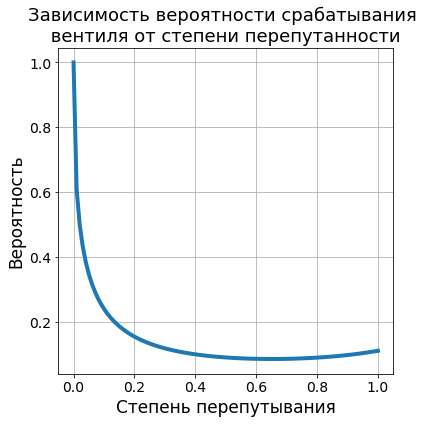
\includegraphics[scale=0.6]{cphase_prob.png}}
\caption{График зависимости вероятности срабатывания оптического перепутывающего двухкубитового вентиля $Cphase(\theta)$ от степени перепутанности $\theta$.} \label{fig:cphase_prob}
\end{figure}

\qquad Модернизация $B_{RY}$ блока с параметризованным двухкубитовым перепутывающим вентилем $B_{Cphase RY}$ предполагается эффективной по ряду причин. В первую очередь, двухкубитовый вентиль с меньшей перепутывающей способностью проще реализовать физически, а, например, при использовании оптической dual rail кодировки при увеличении запутанности параметризованного вентиля уменьшается вероятность его срабатывания (см. рис. \ref{fig:cphase_prob}). Таким образом, в определённых ситуациях использование перепутывающих вентилей с ограниченной перепутывающей способностью может быть полезно. Более того появляется возможность исключить параметр, регулирующий запутывающую способность двухкубитового вентиля, из вектора оптимизируемых параметров и фиксировать его, тем самым ограничивая максимальную запутанность, или же изменять по заданному закону в процессе оптимизации, тем самым динамически изменяя функцию потерь оптимизатора. 

\qquad Блок $B_{RY RZ}$ рассматривается для подтверждения эффективности $B_{RY}$ несмотря на наличие однокубитовых вращений исключительно около оси $Y$ на сфере Блоха.

\newpage

\begin{center}
\section{МОДЕЛИРОВАНИЕ ВАРИАЦИОННЫХ КВАНТОВЫХ АЛГОРИТМОВ} \label{numerical_calculations}
\end{center}

\qquad В настоящей главе проведён анализ эффективности использования вариационных квантовых алгоритмов на основе аппаратно-эффективного анзаца для поиска энергии основного состояния квантовомеханической системы с заданным гамильтонианом. Для анализа эффективности проводится численное моделирование поиска основного состояния нескольких гамильтонианов с использованием вариационных квантовых алгоритмов. В качестве примеров рассмотрены гамильтониан Швингера \cite{Borzenkova_2021}, \cite{Buyens_2016}, гамильтонианы двухатомных молекул $H_2$ и $LiH$, а так же гамильтониан трёхатомной молекулы $H_2O$.


\subsection{Инструменты анализа эффективности}

\qquad Данном параграфе описываются метрики, по которым проводится анализ эффективности анзаца для ВКА. Для сравнения различных архитектур анзаца, способов инициализации начальных параметров, классических оптимизаторов и функций потерь проводится серия запусков оптимизации для оценки статистик на каждый уникальный набор характеристик.

\qquad Далее проводится сравнение наблюдаемой энергии в процессе оптимизации. Так же в зависимости от задачи в процессе оптимизации сохраняются дополнительные величины, такие как значения параметров вариационной схемы или степени запутанности подсистем в процессе оптимизации, полезные для анализа наблюдаемые, связанные с заданным гамильтонианом.

\qquad Эффективность работы ВКА с заданной конфигурацией оценивается по критериям  точности и скорости оптимизации. При этом основным критерием является точность.

\qquad При сравнения точности оптимизации для различных размерностей необходимо учитывать абсолютное значение величины энергии основного состояния для каждой размерности. Чтобы устранить влияние величины абсолютного значения энергии будем рассматривать относительную ошибку:

\begin{equation}
\delta E = \frac{E^{opt}_N - E^{real}_N}{|E^{real}_N|}, 
\end{equation} где $E^{opt}_N$ - значение энергии, найденное при моделировании оптимизации при помощи ВКА; $E^{real}_N$ - теоретическое значение энергии основного состояния.

\qquad При этом для рассматриваемых размерностей теоретическое значение энергии может быть найдено с высокой точностью численно при помощи классического разложения матрицы оператора гамильтониана по собственным векторам:


\begin{equation}
\hat H = \sum_{i = 0}^N \lambda_{i} \vec{\psi}_{i}, \label{eq:delta_E}
\end{equation} где  $\lambda_{i}$ и $\vec{\psi}_{i}$ - собственные значения и собственные вектора матрицы $\hat H$.

\qquad Тогда классическая численная оценка теоретическое значение энергии основного состояния системы с заданным гамильтонианом равна минимальному собственному значению матрицы $\hat H$:

\begin{equation}
E_{min} = min_{i}(\lambda_{i}), 
\end{equation} где $\lambda_{i}$ - собственные значения матрицы $\hat H$.


\qquad Для получения дополнительной информации об эффективности применения конкретного анзаца для поиска основного состояния заданного гамильтониана можно исследовать гиперповерхность оптимизации, заданную зависимостью значений энергии основного состояния от вектора параметров анзаца. В работе \cite{https://doi.org/10.48550/arxiv.2111.04695} представлен способ получения визуальной оценки характеристик гиперповерхности оптимизации путём визуализации и анализа наиболее информативной проекции многомерной гиперповерхности, полученной с использованием метода сокращения размерности.

\qquad Упомянутый способ поиска наиболее информативной проекции гиперповерхности оптимизации основан на применении метода анализа главных компонент (в англоязычной литературе principal component analysis PCA) к набору векторов параметров, представляющему траекторию оптимизации на гиперповерхности. Тогда при помощи анализа главных компонент находится $n$ ортогональных векторов, в направлении которых траектория оптимизации отображает наибольшую дисперсию. В случае $n = 2$ полученные вектора, задают плоскость наиболее информативной проекции гиперповерхности оптимизации.

\begin{figure}[H]
\center{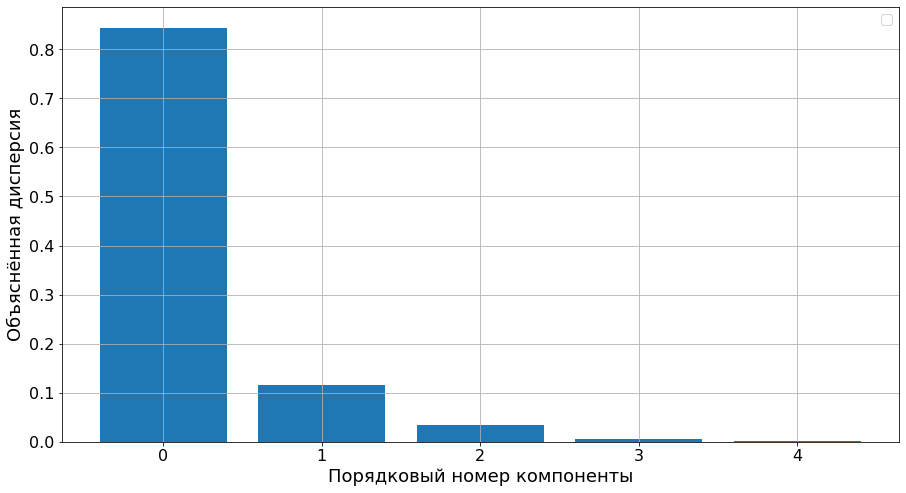
\includegraphics[scale=0.40]{disp_bar_chart.png}}
\caption{Диаграмма, иллюстрирует распределение объясненной дисперсии по базисным векторам, полученным с помощью метода анализа главных компонент для гиперповерхности оптимизации, соответствующей поиску основного состояния гамильтониана Швингера размерности $N = 5$ при помощи аппаратно-эффективного анзаца, основанного на двухкубитовом блоке $B_{RY}$ без блока перестановок глубиной $l = 1$.} \label{fig:disp_bar}
\end{figure}

\qquad Количественной мерой сохранённой информации о многомерной гиперповерхности после проецирования служит доля объяснённой дисперсии соответствующая векторам, задающим плоскость проекции. Согласно рис. \ref{fig:disp_bar} первые две компоненты распределения объяснённой дисперсии по базисным векторам для гиперповерхности оптимизации, соответствующей поиску основного состояния гамильтониана Швингера размерности $N = 5$ при помощи однослойного диагонального анзаца, сохраняют 96\% информации о гиперповерхности оптимизации.

\subsection{Гамильтониан Швингера}

\qquad Гамильтониан Швингера выбран, как базовая модель для оценки эффективности различных конфигураций зацикленных схем ВКА, так как масштабируется на произвольную размерность, имеет сложную структуру связей, при определённых параметрах демонстрирует квантовый фазовый переход, возле которого поиск энергии основного состояния значительно усложняется.

\qquad Модель Швингера описывает взаимодействия между фермионами Дирака через фотоны в двумерном пространстве. В связи с групповым взаимодействием всех частиц волновая волновая функция характеризуется высокой степенью многочастичной запутанности. гамильтониан Швингера описывает рождение и аннигиляцию электрон-позитронных пар, а так же их взаимодействие с учётом массы частиц:

\begin{equation} 
H_{N} = w \sum_{j=1}^{N-1} [\sigma_{j}^{+} \sigma_{j+1}^{-} + H.c.] + \frac{m}{2} \sum_{j=1}^{N} (-1)^{j} \sigma_{j}^{z} - g \sum_{j=1}^{N} L^{2}_{j}.\label{eq:shwinger}
\end{equation} где $\sigma_{j}^{+-} = \sigma_{j}^{x} +- i\sigma_{j}^{y}$, а оператор $L_{j}$ имеет вид:

\begin{equation}
L_{j} = \epsilon_{0} - \frac{1}{2} \sum_{l=1}^{j} [\sigma_{l}^{z} + (-1)^{l}]
\end{equation}

\qquad Гамильтониан Швингера состоит из трех слагаемых: первое отвечает за взаимодействие электрона и позитрона, второе зависит от затравочной массы частиц m, а третье обозначает энергию электрического поля. Мы принимаем коэффициенты $w = g = 1$ и рассматриваем только зависимость основной энергии гамильтониана от массы (см. рис. \ref{fig:Shwinger}). 

\begin{figure}[H]
\begin{minipage}[H]{0.46\linewidth}
\center{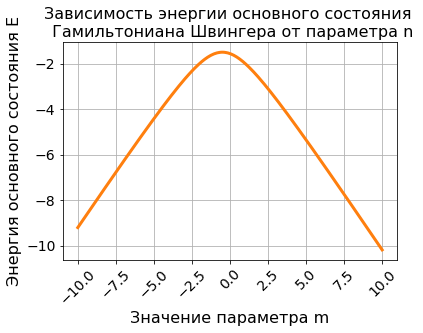
\includegraphics[width=\textwidth]{Shwinger_energy.png} а)}
\end{minipage}
\hfill
\begin{minipage}[H]{0.51\linewidth}
\center{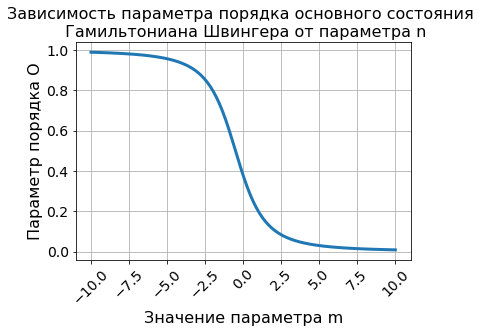
\includegraphics[width=\textwidth]{Shwinger_order_param.png} б)}
\end{minipage}
\caption{Графики аналитической зависимости характеристик модели Швингера от поэлементной массы системы фермионов Дирака для размерности $N = 2$: a) зависимость энергии основного состояния гамильтониана Швингера от массы частиц; б) Зависимость среднего значения наблюдаемой параметра порядка для основного состояния модели Швингера от массы частиц системы.}\label{fig:Shwinger}
\end{figure}

\qquad Наблюдаемая $O$, именуемая параметром порядка, демонстрирует квантовый фазовый переход при варьировании массы частиц (см. рис. \ref{fig:Shwinger}). Известна аналитическая зависимость среднего значения параметра порядка для основного состояния гамильтониана Швингера от размерности, что делает её полезной для дополнительного анализа сходимости вариационного алгоритма к верному решению при анализе эффективности ВКА.

\begin{equation}
\langle O \rangle = \frac{1}{2N(N-1)}\sum_{j>i} \langle (I+(-1)^i \sigma^{z}_{i}) ( 1 + (-1)^{j} \sigma^{z}_{j} \rangle,
\end{equation} где $O$ - параметр порядка,  $\sigma$ - матрицы Паули, $I$ - единичная матрица.

\qquad Рассмотрение относительной ошибки оценки параметра порядка $\delta O = \frac{O^{opt}_N - O^{real}_N}{|O^{real}_N|}$  (по аналогии с формулой \eqref{eq:delta_E}  ) так же может оказаться полезным.

\qquad Далее анализ гамильтониана Швингера будет проводиться только для значения параметра $m=-\frac{1}{2}$, соответствующего фазовому переходу.


\subsection{Выбор метода оптимизации}

\qquad В данной работе для задачи поиска основного состояния гамильтониана Швингера было проведено сравнение двух методов оптимизации АдаМ и КНГ. 

\qquad КНГ показал более высокую скорость сходимости в то время как АдаМ для серии задач показал более высокую точность решения за лучшей счёт способности обходить локальные минимумы (см. рис. \ref{fig:opt_comparence}). Более того для использования АдаМ в отличии от КНГ нет необходимости измерять дополнительные характеристики на квантовом устройстве для реализации оптимизационного процесса, что значительно облегчает физическую реализацию метода.

\qquad Ввиду описанных преимуществ для дальнейшего исследования применяется оптимизатор АdaM.


\begin{figure}[H]
\begin{minipage}[h]{1.\linewidth}
\center{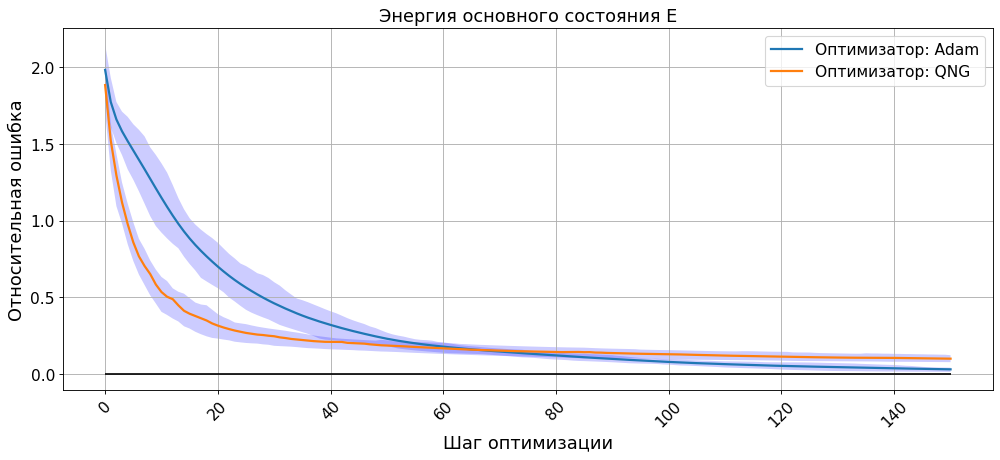
\includegraphics[width=\textwidth]{N9_l3_opt_comparence.png} а)}
\end{minipage}
\vfill
\begin{minipage}[H]{1.\linewidth}
\center{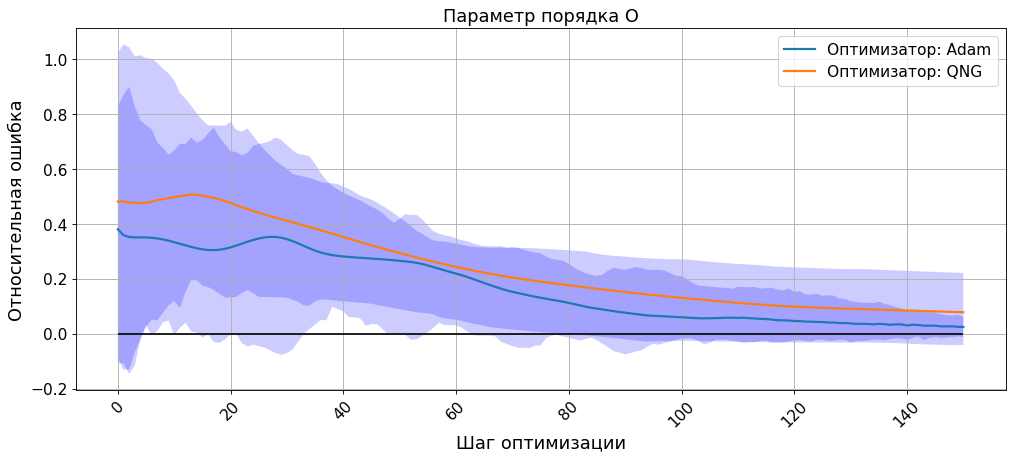
\includegraphics[width=\textwidth]{N9_l3_opt_comparence_O.png} б)}
\end{minipage}
\caption{Графики демонстрирует значения величины относительной ошибки оценок наблюдаемых (а) энергии, (б) параметра порядка основного состояния гамильтониана Швингера размерности $N$ = 9, c использованием аппаратно-эффективного анзаца, основанного на двухкубитовом блоке $B_{RY}$ без блока перестановок между слоями. Используются два различных оптимизатора адаптивная оценка моментов (синяя линия) и квантовый натуральный градиент (оранжевая линия). Линии соответствуют зависимостям средних значений относительной ошибки оценки наблюдаемой на данной итерации за 50 запусков оптимизационного алгоритма со случайно выбранными начальными параметрами. Границы полупрозрачной области около линий соответствуют квантилям значений относительной ошибки оценки наблюдаемой на данной итерации за 50 запусков оптимизационного алгоритма со случайно выбранными начальными параметрами. }\label{fig:opt_comparence}
\end{figure}


\begin{figure}[H]
\begin{minipage}[H]{1.\linewidth}
\center{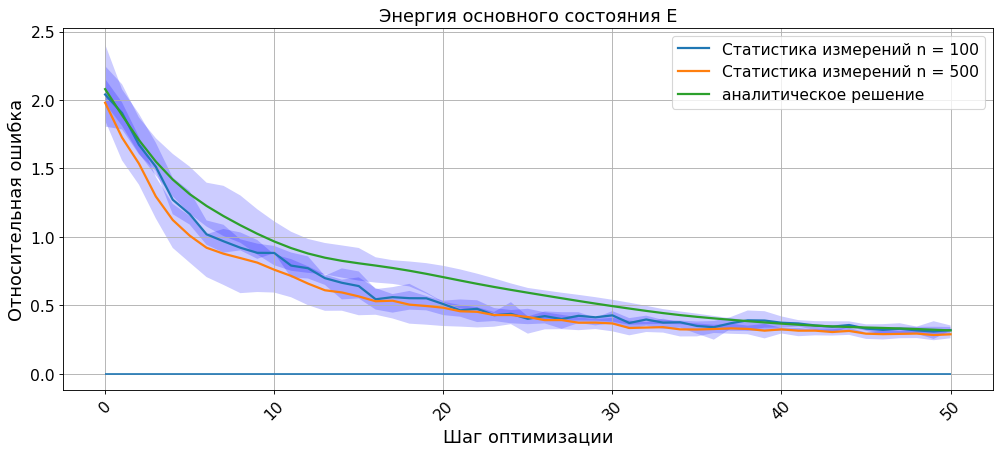
\includegraphics[width=\textwidth]{shots_statistics_optim1.png} а)}
\end{minipage}
\vfill
\begin{minipage}[H]{1.\linewidth}
\center{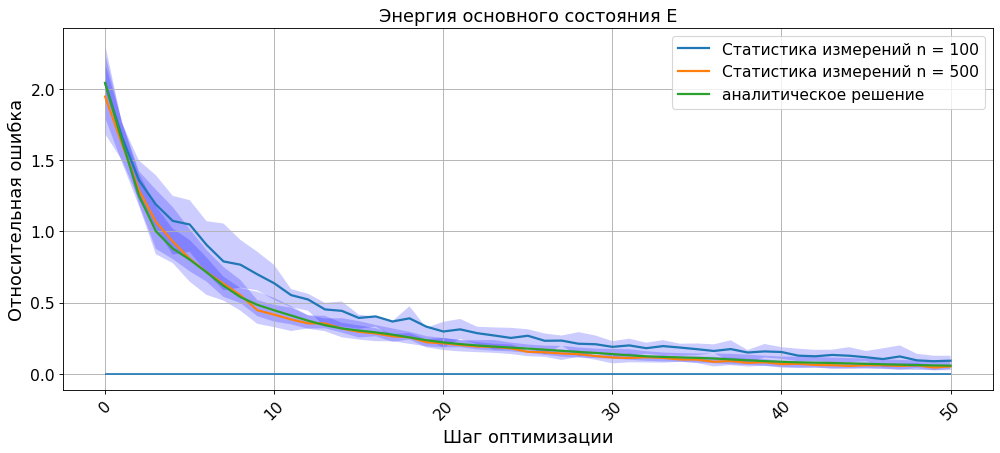
\includegraphics[width=\textwidth]{shots_statistics_optim.png} б)}
\end{minipage}
\caption{Графики демонстрирует значения величины относительной ошибки оценки энергии основного состояния гамильтониана Швингера размерности $N = 5$ в процессе оптимизации с использованием аппаратно-эффективного анзаца, основанного на двухкубитовом блоке $B_{RY}$ без блока перестановок для различных размеров статистики оценки наблюдаемой. Рассматривается анзац глубиной (a) $l = 1$, (б) $l = 4$ слоёв. Синяя, оранжевая и зелёная линии на графиках соответствуют оптимизации с объёмом статистики измерений для каждой наблюдаемой 100, 500 запусков и аналитической оценке. Линии соответствуют зависимостям средних значений относительной ошибки оценки наблюдаемой на данной итерации за 50 запусков оптимизационного алгоритма со случайно выбранными начальными параметрами. Границы полупрозрачной области около линий соответствуют квантилям значений относительной ошибки оценки наблюдаемой на данной итерации за 50 запусков оптимизационного алгоритма со случайно выбранными начальными параметрами.}\label{fig:shots_comp}
\end{figure}

\subsection[Зависимость точности оценки от размера статистики]{Зависимость точности оценки от размера \linebreak статистики}

\qquad Оценка средних величин наблюдаемой производится на основе набора статистики измерений на заданной квантовой схеме, соответственно относительная ошибка полученного результата зависит от размера статистики измерений, выделенного на каждую наблюдаемую.

\qquad Для анализа рассмотрены статистики измерений объёмом 100, 500 и 1000. 5000 запусков на каждую наблюдаемую и аналитическая оценка наблюдаемой для анзацев глубиной $l=1$ и $l=4$ слоя для поиска энергии основного состояния гамильтониана Швингера размерности $N = 5$. Согласно рис.\ref{fig:shots_comp} для однослойного анзаца процесс оптимизации совпадает при различных объёмах статистики, в то время как для анзаца глубиной $l=4$ слоя наблюдается повышение точности оптимизации при увеличении объёма статистики.


\begin{figure}[H]
\begin{minipage}[H]{0.49\linewidth}
\center{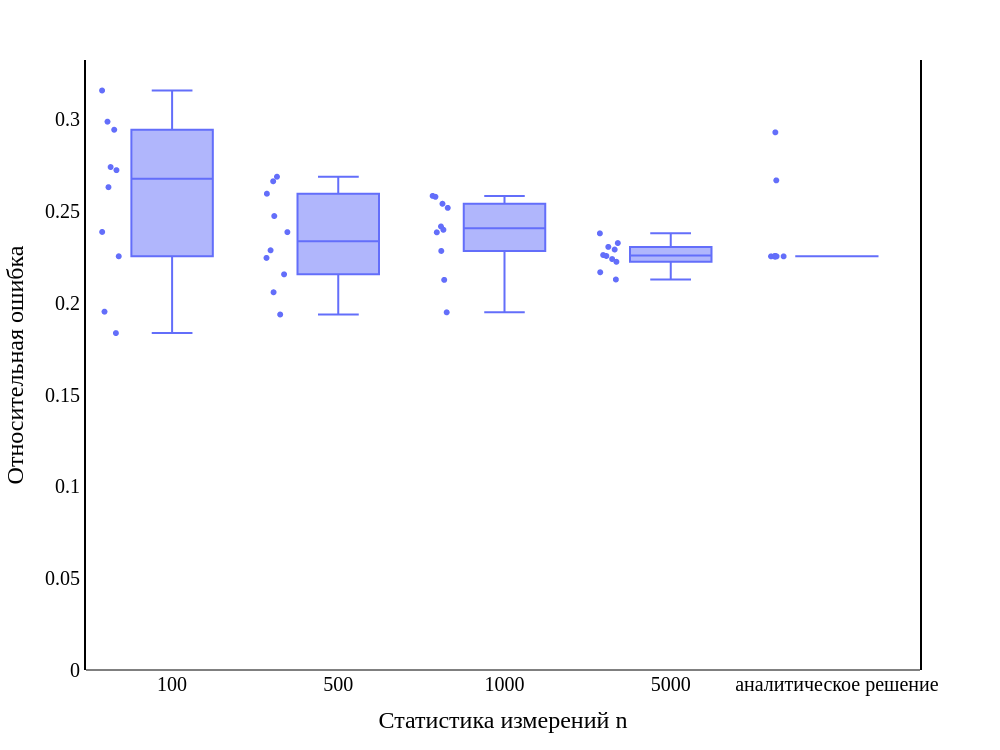
\includegraphics[width=\textwidth]{shots_statistics_end1.png}}
\end{minipage}
\hfill
\begin{minipage}[H]{0.49\linewidth}
\center{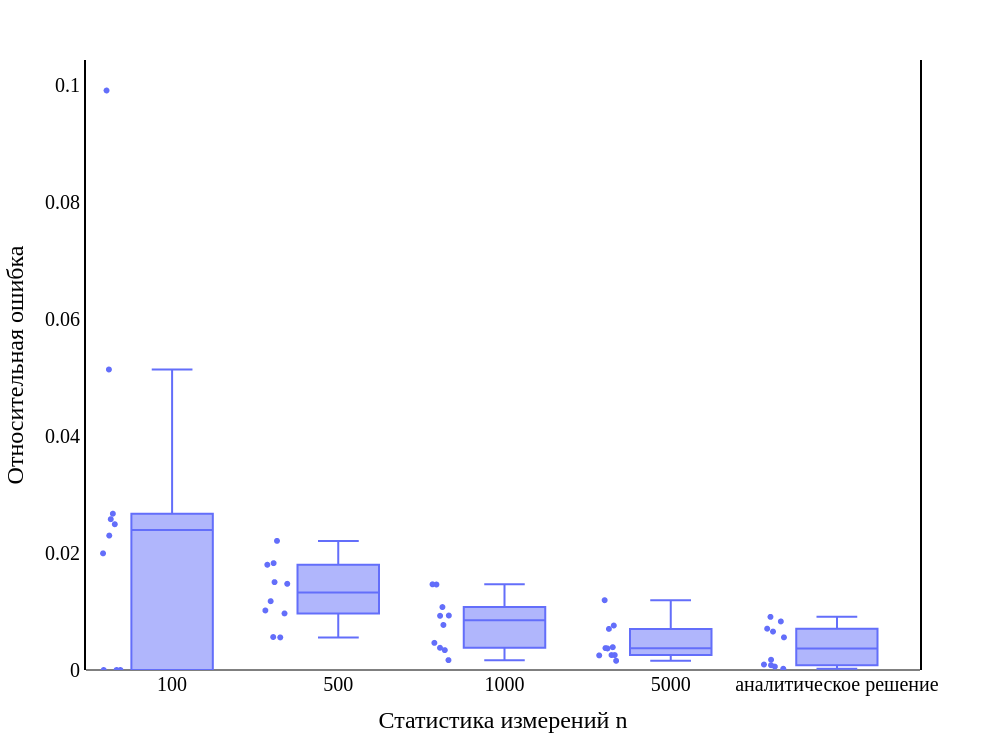
\includegraphics[width=\textwidth]{shots_statistics_end.png}}
\end{minipage}
\caption{Иллюстрация демонстрирует итоговое распределение величины относительной ошибки оценки энергии основного состояния гамильтониана Швингера размерности $N = 5$ с использованием аппаратно-эффективного аназаца, основанного на двухкубитовом блоке $B_{RY}$ без блока перестановок глубиной (a) $l = 1$ (б) $l = 4$ слоёв с различным объёмом статистики измерений для каждой наблюдаемой. Рассматриваются размеры выборки 100, 500 и 1000, 5000 запусков и аналитическая оценка.}\label{fig:shots_comp_res}
\end{figure}

\qquad Аналогичные выводы можно сделать из рис. \ref{fig:shots_comp_res}. Видно, что итоговое распределение относительной ошибки для однослойного анзаца сопоставимо по среднему значению, а при увеличении объёма выборки лишь уменьшается дисперсия распределения относительной ошибки для серии запусков процесса оптимизации. Большая ошибка связана с невозможностью приготовления основного состояния сильно смешанной системы с помощью однослойной схемы ввиду одномерной геометрии связей. При этом гиперповерхность оптимизации достаточно простая для нахождения глобального минимума при помощи грубой оценки наблюдаемой на каждой итерации с использованием статистики малого объёма. Рассмотрение итогового распределения относительной ошибки для анзаца глубиной $l = 4$ слоя демонстрирует, что точность значительно возрастает при увеличении объёма статистики измерений на оценку наблюдаемой. Основное состояние заданного гамильтониана может быть приготовлено с помощью многослойного анзаца, при этом значительно усложняется гиперповерхность оптимизации, в результате чего для поиска основного состояния необходимо использовать статистику измерений большего объёма для получения оценок наблюдаемой с меньшей дисперсией.

\qquad Далее в работе рассматривается только аналитическая оценка наблюдаемых, в предположении, что для заданной схемы в зависимости от её глубины и размерности рассматриваемой системы можно подобрать достаточный объём выборки для получения оценки наблюдаемой с наперёд заданной близостью к аналитическому значению.


\subsection[Зависимость точности оценки от количества слоёв и размерности квантовой схемы]{Зависимость точности оценки от количества \linebreak слоёв и размерности квантовой схемы}

\qquad При увеличении размерности рассматриваемой квантовой системы даже использование в качестве двухкубитового блока универсального блока, готовящего произвольное двухкубитовое состояние не позволяет приготовить произвольное многокубитовое состояние при простом попарном их объединении. Зацикленные оптические схемы с повторным использованием физических кубитов позволяют рассматривать многослойные структуры, при этом добавление каждого логического слоя значительно усложняет физическую реализацию, а в рассматриваемом случае оптической dual rail кодировки снижает вероятность срабатывания. Таким образом, важным вопросом становится подбор оптимальной глубины анзаца, для достижения желаемой точности оптимизации.

\begin{figure}[H]
\center{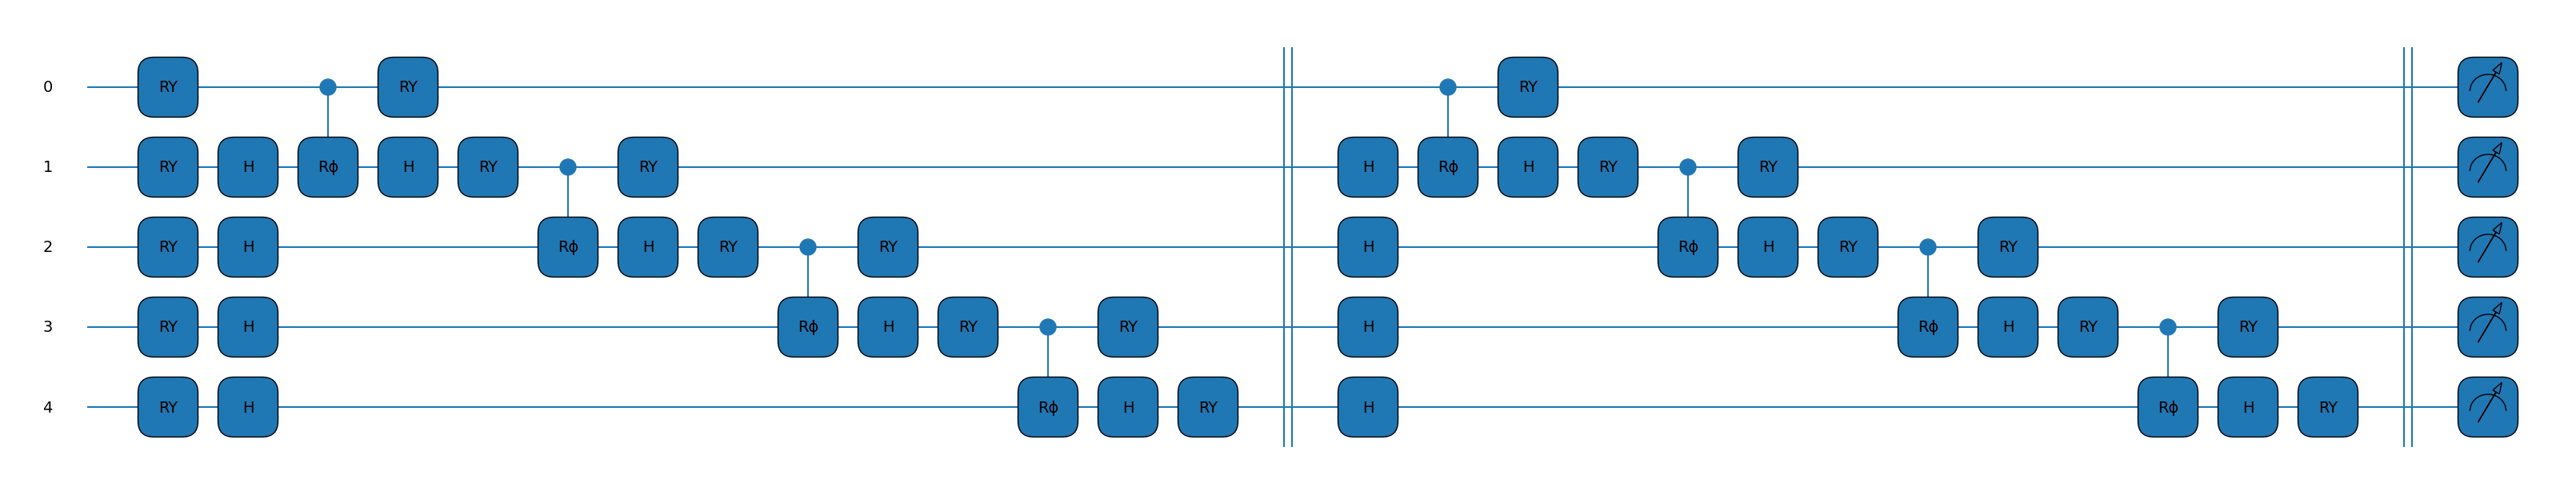
\includegraphics[scale=0.2]{layered_ansatz_naive.png}}
\caption{Блок-схема, иллюстрирует общий вид аппаратно-эффективного анзаца, основанного на двухкубитовом блоке $B_{RY}$ без блока перестановок. На рисунке представлен анзац размерности $N=5$ глубиной $l=3$ слоя без перестановочных блоков между слоями. Перепутывающие вентили $Cphase(\theta)$ зафиксированы в максимально перепутанном состоянии $\theta = \pi$.} \label{fig:Cphase_HEA_ansatz}
\end{figure}

\qquad Для поиска зависимости точности оптимизации от размерности системы кубитов и глубины анзаца рассмотрим диагональные анзацы, которые возможно реализовать при помощи зацикленных оптических схем без перестановочных блоков. Проведём численное моделирование поиска основного состояния гамильтониана Швингера размерностей $N = 3, 5, 6, 7, 9$ с использованием анзаца глубиной $l = 1, 3, 6, 9$, набрав статистику в 50 запусков оптимизационного алгоритма для каждой комбинации параметров. 

\begin{figure}[H]
\begin{minipage}[H]{0.48\linewidth}
\center{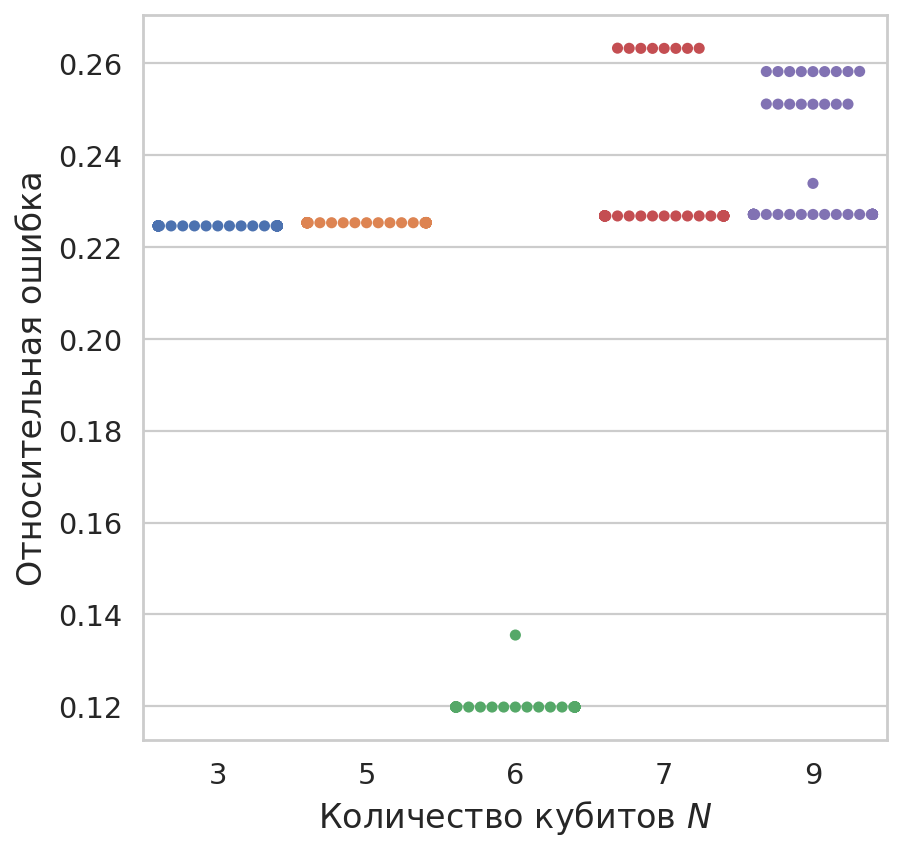
\includegraphics[width=\textwidth]{fidelity_shwinger_l1.png} а) Глубина 1 слой}
\end{minipage}
\hfill
\begin{minipage}[H]{0.48\linewidth}
\center{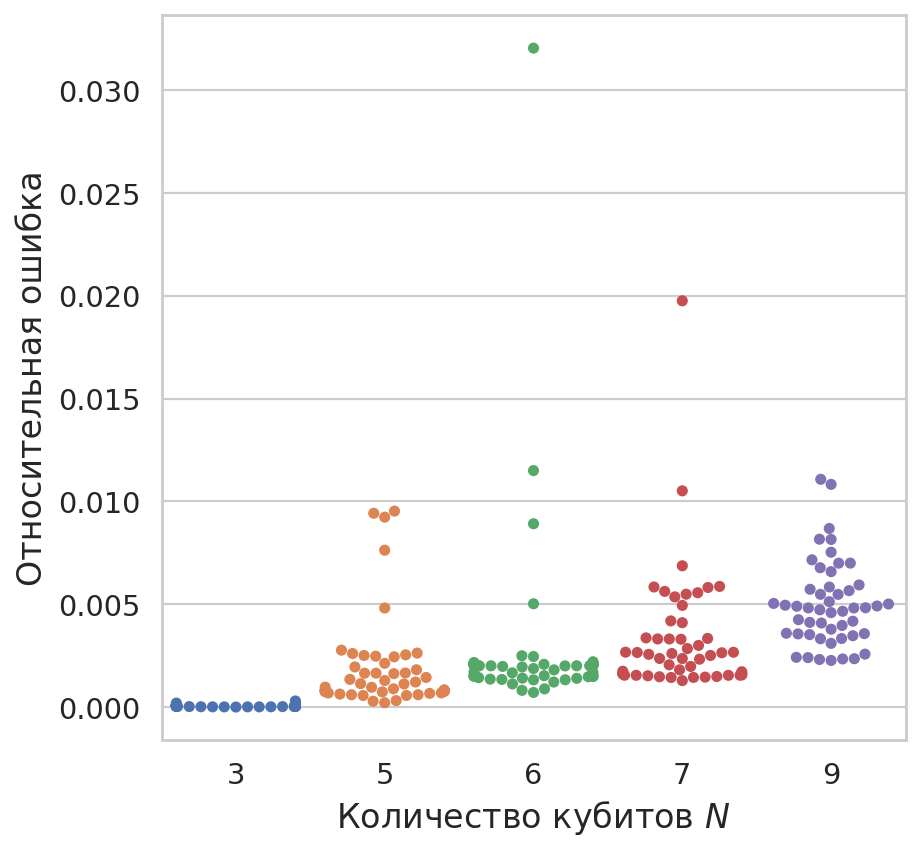
\includegraphics[width=\textwidth]{fidelity_shwinger_l3.png} б) Глубина 3 слоя}
\end{minipage}
\vfill
\begin{minipage}[H]{0.48\linewidth}
\center{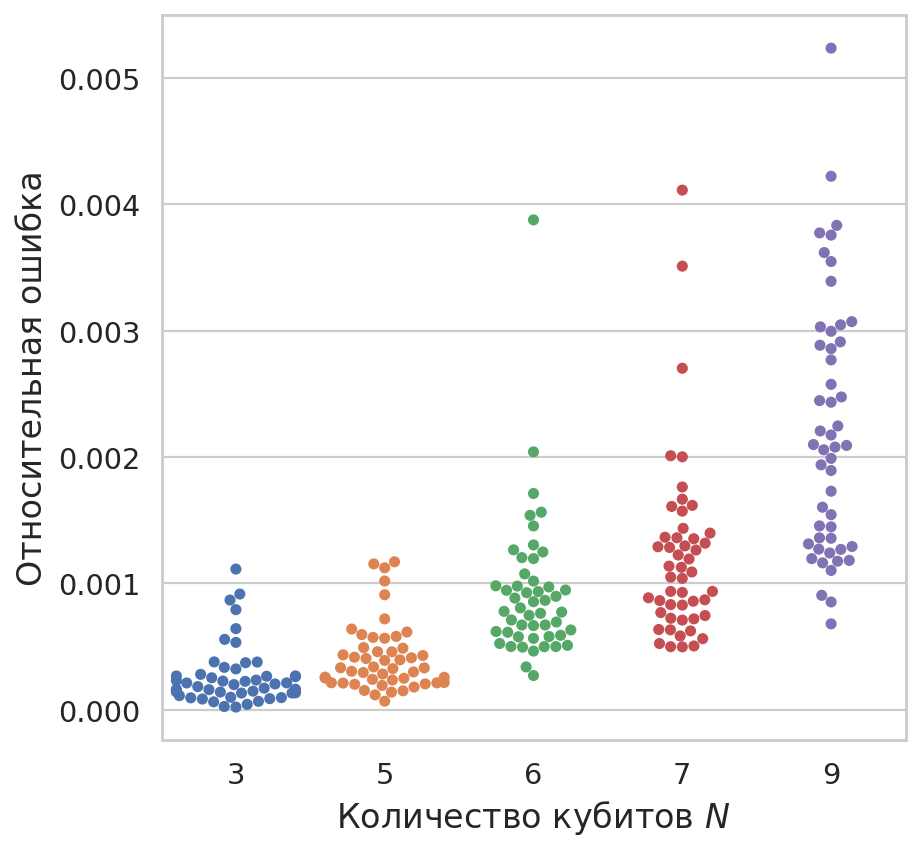
\includegraphics[width=\textwidth]{fidelity_shwinger_l6.png} в) Глубина 6 слоев}
\end{minipage}
\hfill
\begin{minipage}[H]{0.48\linewidth}
\center{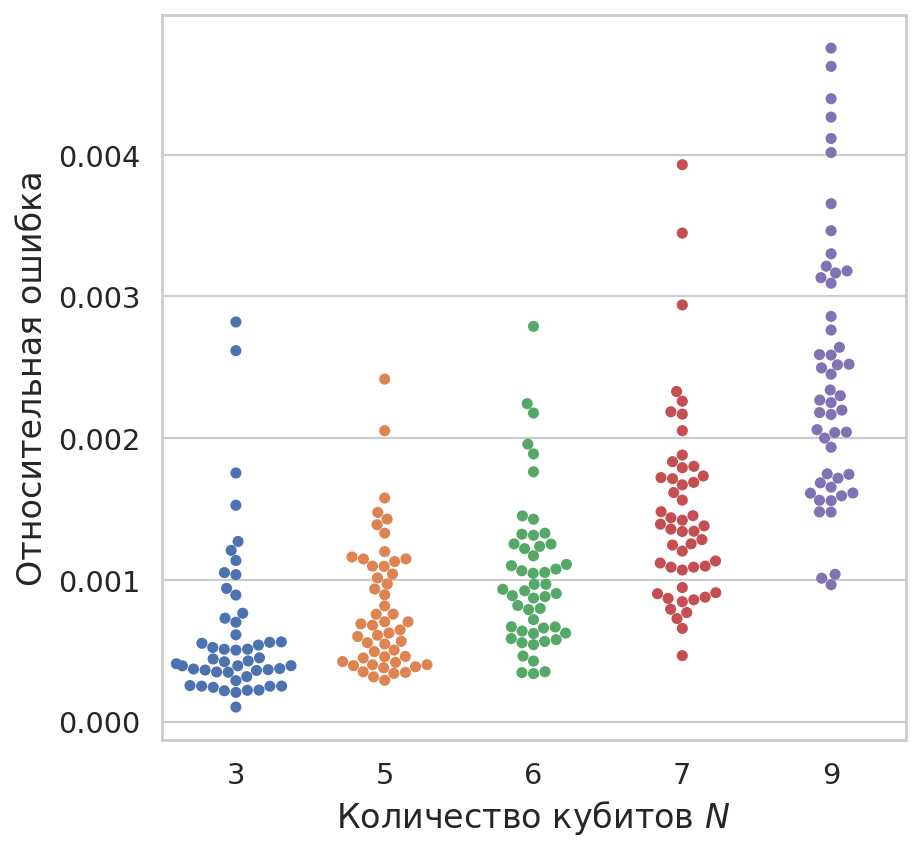
\includegraphics[width=\textwidth]{fidelity_shwinger_l9.png} г) Глубина 9 слоев}
\end{minipage}
\caption{Иллюстрация демонстрирует зависимость распределений относительной ошибки рассчитанных значений энергии основного состояния гамильтониана Швингера от размерности гамильтониана $N$ с использованием аппаратно-эффективного анзаца, основанного на двухкубитовом блоке $B_{RY}$ без блока перестановок с различной глубиной $l = 1, 3, 6, 9$ на графиках а), б), в), г) соответственно.}\label{fig:fidelity_dims}
\end{figure}


\qquad Графики, представленные на рис. \ref{fig:fidelity_dims} демонстрируют зависимость относительной ошибки рассчитанного значения энергии основного состояния в серии запусков оптимизационного процесса от размерности квантовой схемы для схем с различной глубиной. Согласно рис. \ref{fig:fidelity_dims} а) однослойная схема даёт очень грубую оценку искомого основного состояния энергии с ошибкой порядка 20\% от абсолютного значения для размерностей $N$ = 3,5,7,9 и 10\% от абсолютного значения для размерности $N$ = 6. Отличие для размерности $N$ = 6 вероятно связано с особенностью гамильтониана Швингера для чётной размерности описываемой системы частиц. Низкая точность оценки энергии основного состояния по видимому связана с тем, что невозможно реализовать преобразование, готовящее состояние, соответствующее искомому основному состоянию энергии, в виду одномерной связи между кубитами (каждый напрямую связан только с соседними).




\begin{figure}[H]
\begin{minipage}[H]{0.48\linewidth}
\center{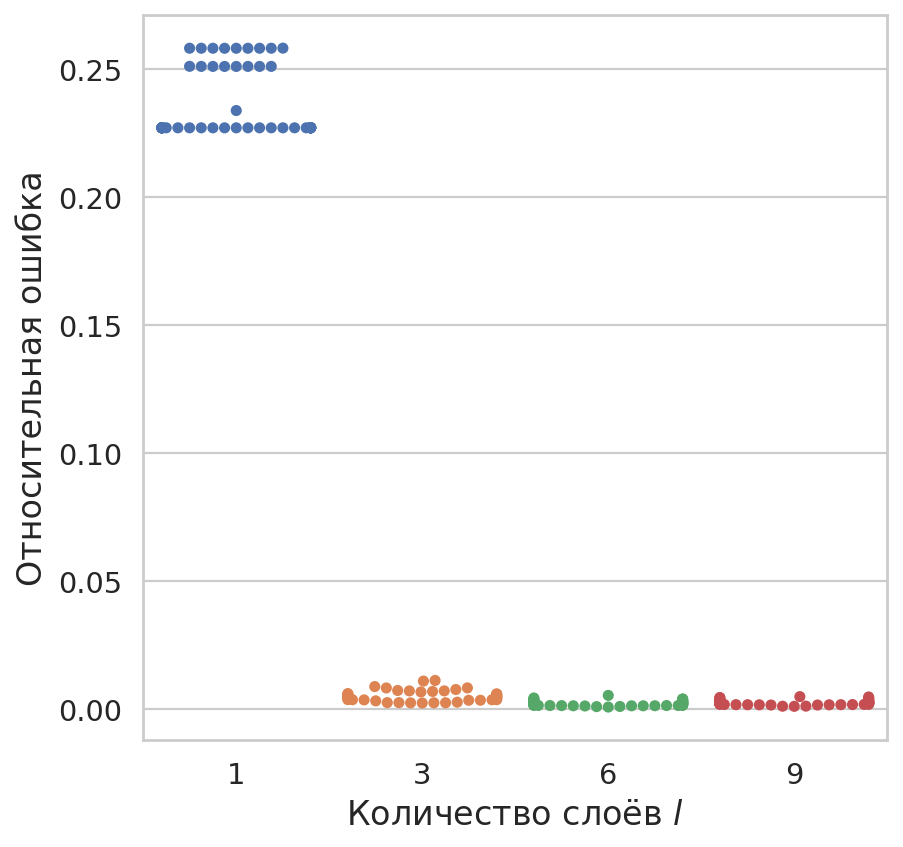
\includegraphics[width=\textwidth]{fidelity_shwinger_N9l1369.png} а)}
\end{minipage}
\hfill
\begin{minipage}[H]{0.48\linewidth}
\center{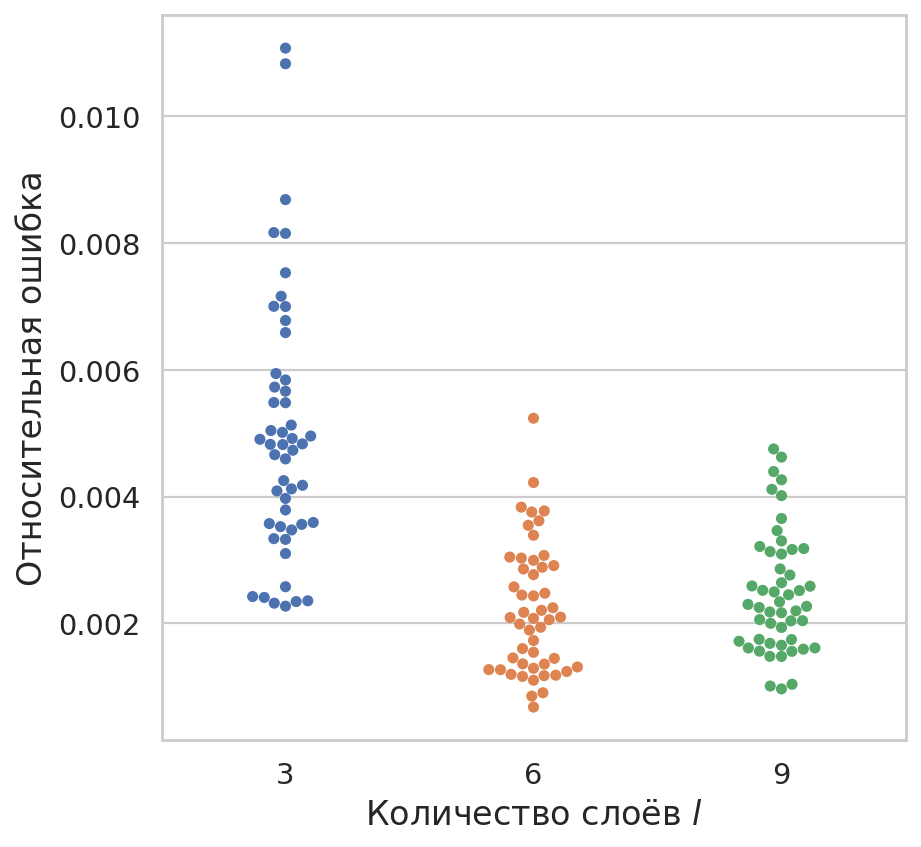
\includegraphics[width=\textwidth]{fidelity_shwinger_N9l369.png} б)}
\end{minipage}
\caption{Иллюстрация демонстрирует зависимость распределений относительной ошибки оценки энергии основного состояния гамильтониана Швингера размерности $N = 9$ от глубины аппаратно-эффективного анзаца, основанного на двухкубитовом блоке $B_{RY}$ без блока перестановок каналов. а) На графике представлено сравнение для анзацев глубины $l = 1,3,6,9$; б) yа графике отдельно представлено сравнение для анзацев глубины $l = 3,6,9$ в увеличенном масштабе.}\label{fig:fidelity_layers}
\end{figure}

\qquad Использование многослойных схем решает проблему недостаточной экспрессивности анзаца и моделирование процесса оптимизации с анзацами с глубиной $l=3,6,9$ слоёв показывает высокую точность оценки величины значения энергии основного состояния с ошибкой в диапазоне от 0.1\% до 1\% от абсолютного значения. При этом сравнение графиков \ref{fig:fidelity_dims}(в) и \ref{fig:fidelity_dims}(г) демонстрирует, что для рассматриваемых размерностей и глубин схем максимальная точность достигается на глубине схемы  $l=6$ слоёв, это связано с усложнением процесса оптимизации при увеличении количества оптимизируемых параметров при добавлении новых слоёв. Таким образом для задачи определённой размерности можно найти оптимальною глубину квантовой схемы для поиска основного состояния системы.

\qquad Аналогичные выводы можно сделать на основании рис. \ref{fig:fidelity_layers}, который демонстрирует зависимость относительной ошибки оценки основного состояния энергии гамильтониана от количества слоёв используемого анзаца.

\subsection[Сравнение двухкубитовых перепутывающих блоков]{Сравнение двухкубитовых перепутывающих \linebreak блоков}

\qquad Двухкубитовый перепутывающий блок рекуррентно используется с помощью зацикленной схемы для реализации многокубитовой логической схемы. Аналитического расчёт характеристик логической схемы для заданного двухкубитового блока не представляется возможным, в связи с чем для подбора блока, реализующего наиболее эффективную схему, проводится моделирование поиска основного состояния системы с использованием анзацев, составленных на основе различных двухкубитовых блоков.

\qquad В данной работе для анализа эффективности выбраны двухкубитовые блоки, представленные на рис. \ref{fig:block_comp}. Проводится моделирование поиска основного состояния гамильтониана Швингера размерности $N = 5$ с использованием анзацев глубиной $l = 1$ и $l = 4$ слоёв для различных двухкубитовых блоков.


\begin{figure}[H]
\begin{minipage}[H]{1.\linewidth}
\center{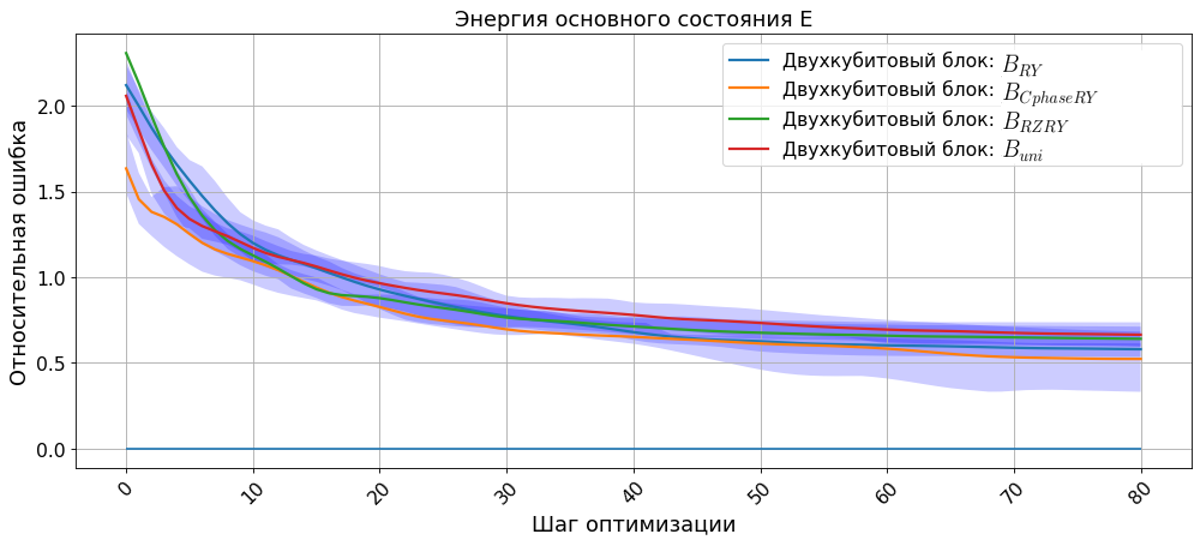
\includegraphics[width=\textwidth]{block_HEA_1l_ly.png} а)}
\end{minipage}
\vfill
\begin{minipage}[H]{1.\linewidth}
\center{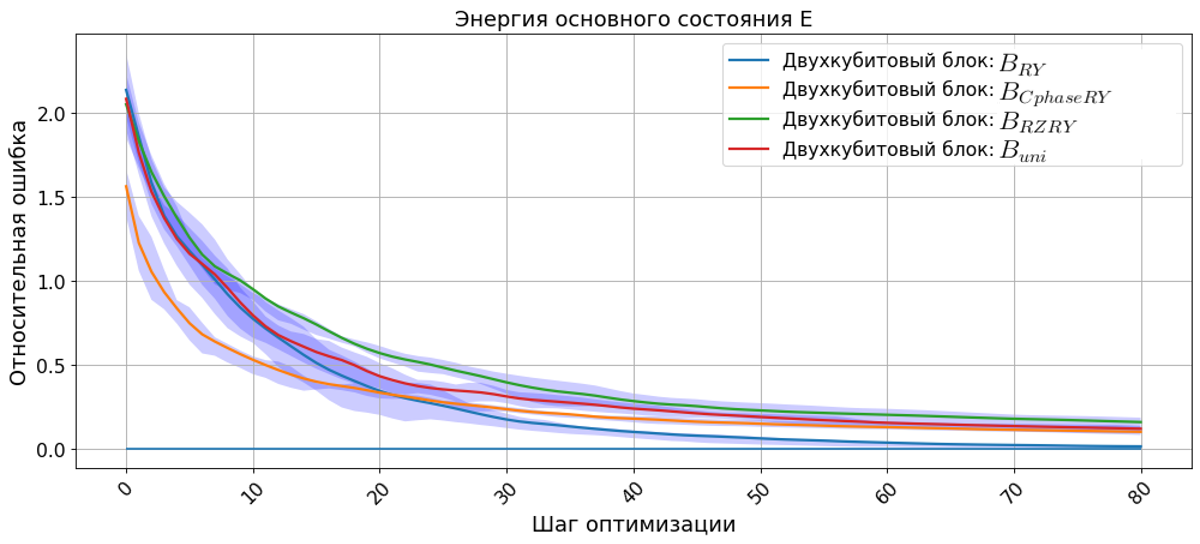
\includegraphics[width=\textwidth]{block_HEA_4l_ly.png} б)}
\end{minipage}
\caption{Графики демонстрируют значения величины относительной ошибки оценки энергии основного состояния гамильтониана Швингера размерности $N = 5$ в процессе оптимизации при помощи аппаратно-эффективного анзаца без блоков перестановки каналов для различных двухкубитовых перепутывающих блоков при глубине схемы a) $l = 1$, б) $l = 4$ слоёв. Синяя, оранжевая, зелёная и красная линии на графиках соответствуют оптимизацию с использованием двухкубитовых перепутывающих блоков $B_{RY}$, $B_{Cphase RY}$, $B_{RY RZ}$ и универсального $B_{uni}$. Линии соответствуют зависимостям средних значений относительной ошибки оценки наблюдаемой на данной итерации за 50 запусков оптимизационного алгоритма со случайно выбранными начальными параметрами. Границы полупрозрачной области около линий соответствуют квантилям значений относительной ошибки оценки наблюдаемой на данной итерации за 50 запусков оптимизационного алгоритма со случайно выбранными начальными параметрами.}\label{fig:mix_block_comp}
\end{figure}


\qquad Сравнение эффективности анзацев на основе анализируемых двухкубитовых перепутывающих блоков показало, что наилучшая точность достигается при использовании двухкубитового перепутывающего $B_{RY}$ блока (см. рис. \ref{fig:mix_block_comp}), отличающей чертой которого является низкая экспрессивность. При использовании однослойного анзаца все анализируемые блоки показали сопоставимые результаты с высокой относительной ошибкой $\delta E \approx 0.5$ от абсолютного значения (см. рис. \ref{fig:mix_block_comp}(а)), что обосновано одномерной геометрией связи между блоками, которая не позволяет приготовить многокубитовое состояние с высокой запутанностью с помощью однослойной схемы вне зависимости от используемых двухкубитовых запутывающих блоков.

\begin{figure}[H]
\begin{minipage}[H]{0.49\linewidth}
\center{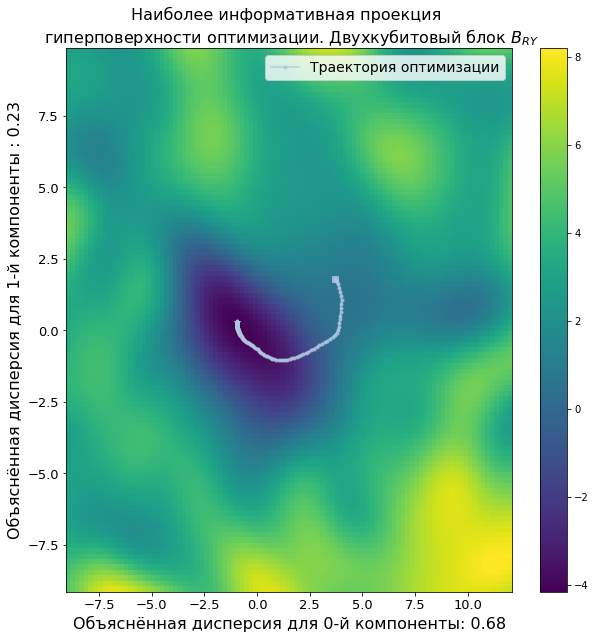
\includegraphics[width=\textwidth]{HEA_4l_surface.png} а)}
\end{minipage}
\hfill
\begin{minipage}[H]{0.49\linewidth}
\center{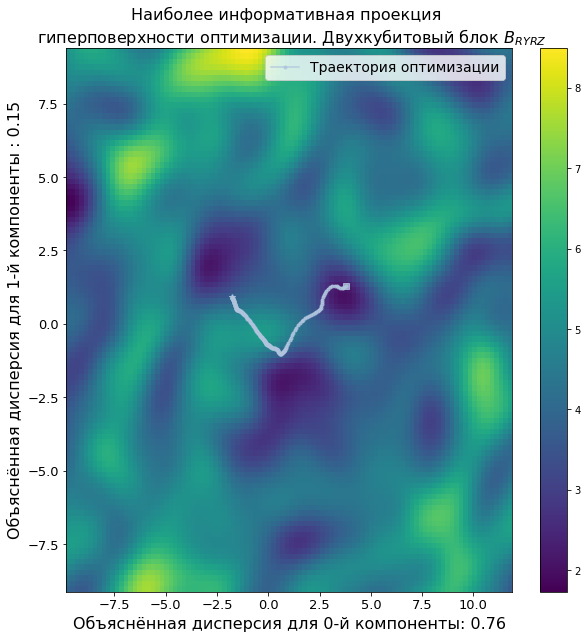
\includegraphics[width=\textwidth]{HEA_RZ_4l_surface.png} б)}
\end{minipage}
\vfill
\begin{center}
\begin{minipage}[H]{0.49\linewidth}
\center{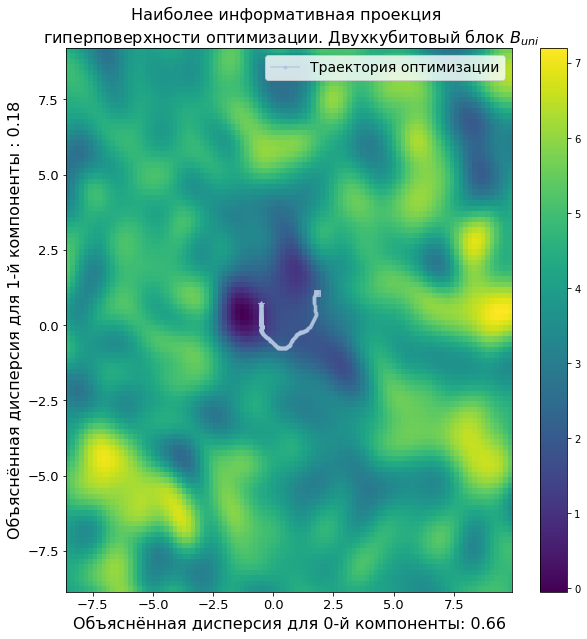
\includegraphics[width=\textwidth]{uni_4l_surface.png} в)}
\end{minipage}
\end{center}
\caption{Иллюстрация демонстрирует сравнение наиболее информативных проекций гиперповерхности оптимизации соответствующей поиску энергии основного состояния гамильтониана Швингера размерности $N = 5$ c применением аппаратно-эффективного анзаца глубиной $l = 4$ слоя без блоков перестановок в зависимости от выбранного двухкубитового перепутывающего блока: а) $B_{RY}$ перепутывающий блок, использующий только однокубитовые вращения только относительно оси $Y$ сферы Блоха $RY (\vec \theta)$ и двухкубитового $CX$; б) $B_{RY RZ}$ с добавлением дополнительных $RZ (\vec \theta)$ вентилей; в) $B_{uni}$ соответствующий универсальному двухкубитовому преобразованию.}\label{fig:proj_comp_block_unit}
\end{figure}


\qquad Анализ многослойного анзаца с глубиной $l = 4$ слоя, способного приготовить многокубитовое состояние с высокой запутанностью, позволяет продемонстрировать преимущество $B_{RY}$ блока. Для анзаца с глубиной $l = 4$ слоя точного решения (относительная ошибка менее $\delta E < 0.01$) позволяет достичь только анзац на основе $B_{RY}$ двухкубитовых блоков. Для анзацев на основе более экспрессивных двухкубитовых блоков процесс оптимизации становится значительно сложнее, ввиду расширения рассматриваемого пространства оптимизации, в результате чего оптимизация останавливается в локальном минимуме, либо на БП в точке, соответствующей результату с относительной ошибкой $\delta E \approx 0.2$. 

\qquad Утверждение об усложнении гиперповерхности оптимизации для анзацев на основе двухкубитовых $B_{RZ_RY}$ и $B_{uni}$ подтверждается, при рассмотрении наиболее информативных проекций соответствующих гиперповерхностей на рис. \ref{fig:proj_comp_block_unit}. Помимо заметного визуального усложнения проекции гиперповерхности для анзацев на основе двухкубитовых $B_{RZ RY}$ и $B_{uni}$ заметим, что суммарная доля объяснённой дисперсии для рассмотренных проекций максимальна для анзаца на основе $B_{RY}$ блока и равняется $92.5\%$. Для блоков $B_{RZ RY}$ и $B_{uni}$ доля суммарной объяснённой дисперсии равна $84\%$ и $91\%$ соответственно, что указывает на более прямолинейную траекторию оптимизации для анзаца на основе $B_{RY}$ блока, и как следствие, её простоту.


\subsection{Сравнение блоков перестановки}

\qquad Блок перестановок между слоями в рассматриваемом виде анзацев позволяет изменить попарные связи между кубитами внутри слоя изменив очерёдность их запутывания и не меняя при этом схему двухкубитового перепутывающего блока. В результате блок перестановок изменяет форму многомерной гиперповерхности параметров, в которой проводится оптимизация, что может в итоге повлиять на точность оптимизации.

\begin{figure}[H]
\begin{minipage}[H]{1.\linewidth}
\center{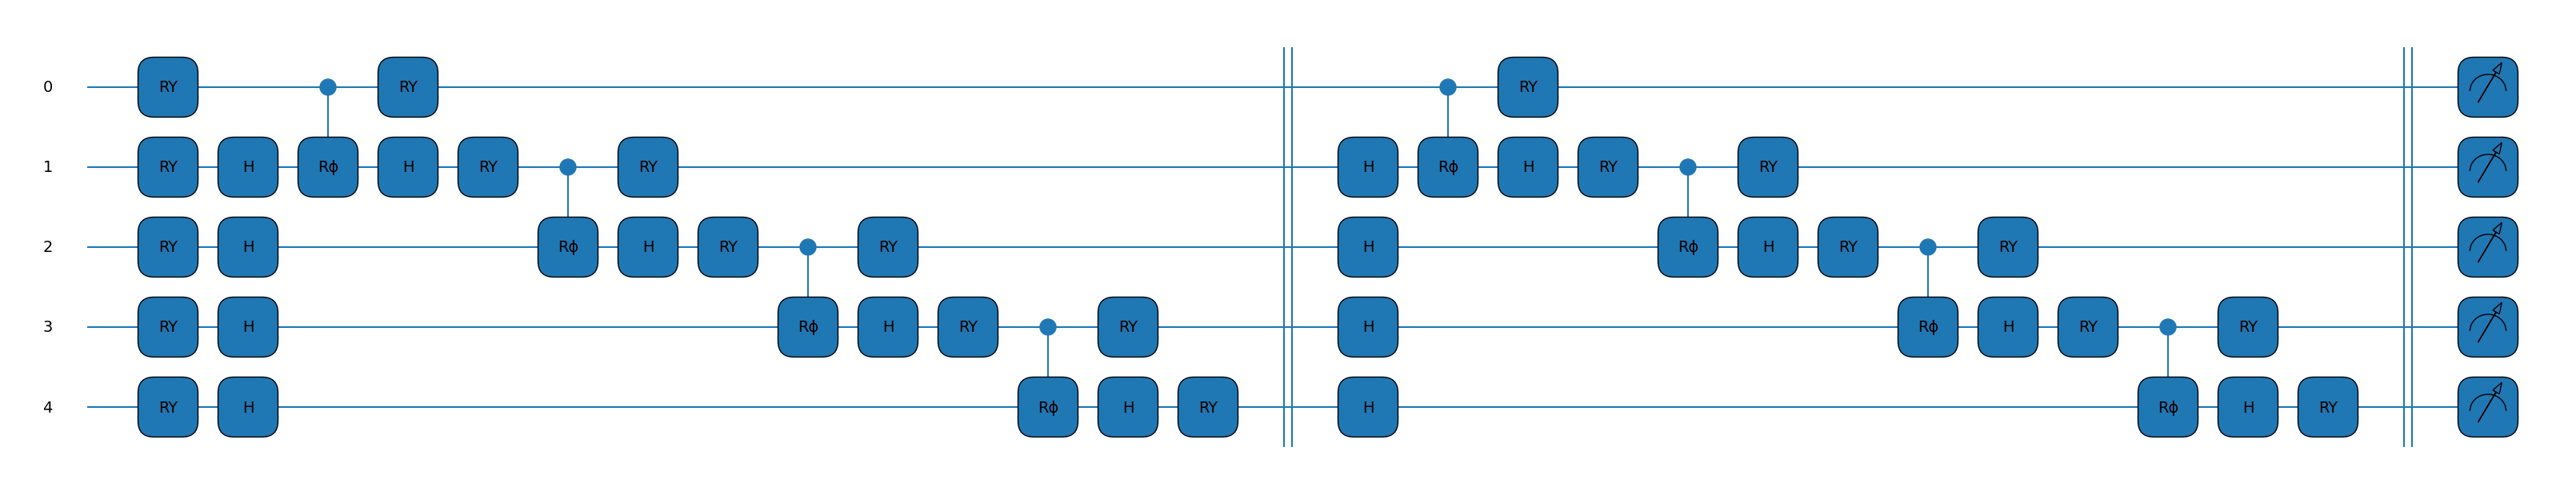
\includegraphics[width=\textwidth]{layered_ansatz_naive.png} а)}
\end{minipage}
\vfill
\begin{minipage}[H]{1.\linewidth}
\center{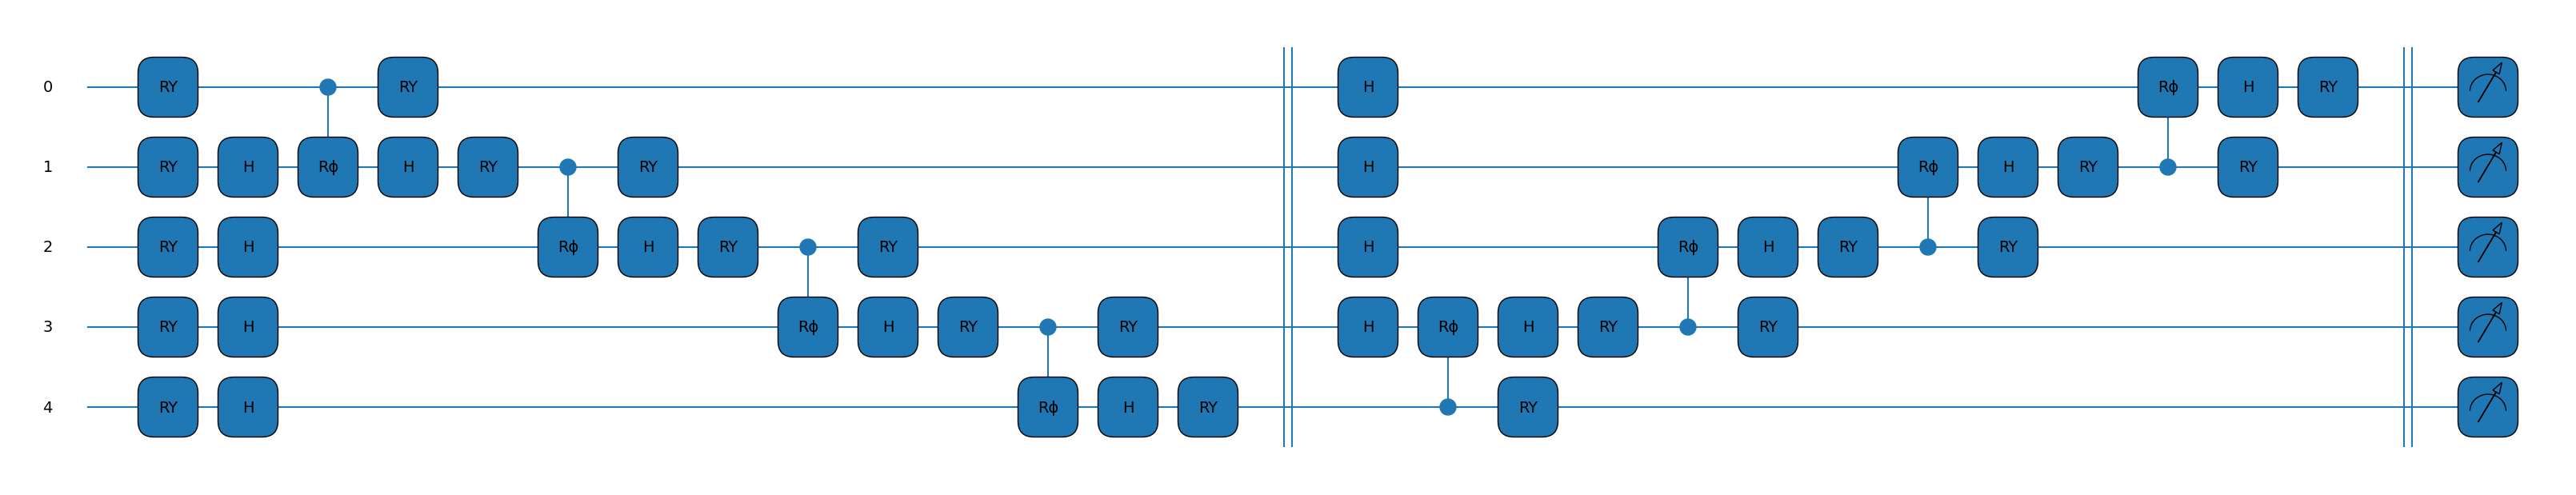
\includegraphics[width=\textwidth]{layered_ansatz_reflected.png} б)}
\end{minipage}
\vfill
\begin{minipage}[H]{1.\linewidth}
\center{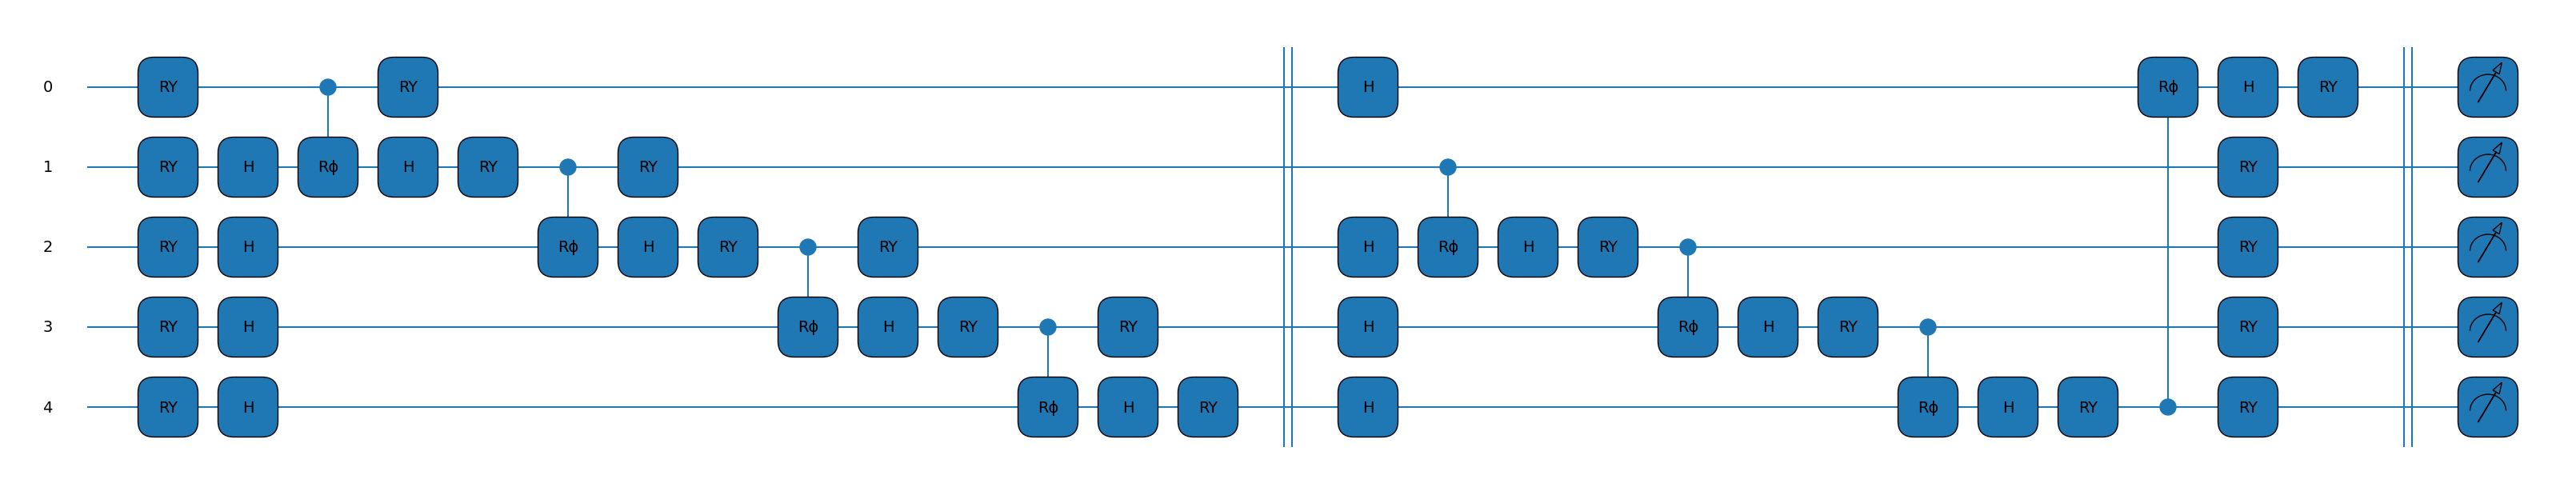
\includegraphics[width=\textwidth]{layered_ansatz_shift1.png} в)}
\end{minipage}
\caption{Блок-схемы, иллюстрируют общий вид аппаратно-эффективного анзаца, основанного на двухкубитовом блоке $B_{RY}$, с различными блоками перестановок: (а) блок перестановок отсутствует, (б) Отражающий блок перестановок после каждого слоя, (в) Блок циклического сдвига на 1 канал после каждлго слоя.}\label{fig:permutation_block}
\end{figure}

\qquad В данном параграфе рассматривается влияние выбора блока перестановок между слоями на среднюю точность получаемого решения. Рассмотреть всевозможные виды перестановочных блоков не представляется возможным, так как их количество комбинаторно возрастает с ростом размерности $N$ системы кубитов. В связи с этим для анализа были выбраны только блоки перестановок осуществляющих отражение каналов и их циклический сдвиг на заданное число $n$ (см. рис. \ref{fig:permutation_block}).

\begin{figure}[H]
\begin{minipage}[H]{1.\linewidth}
\center{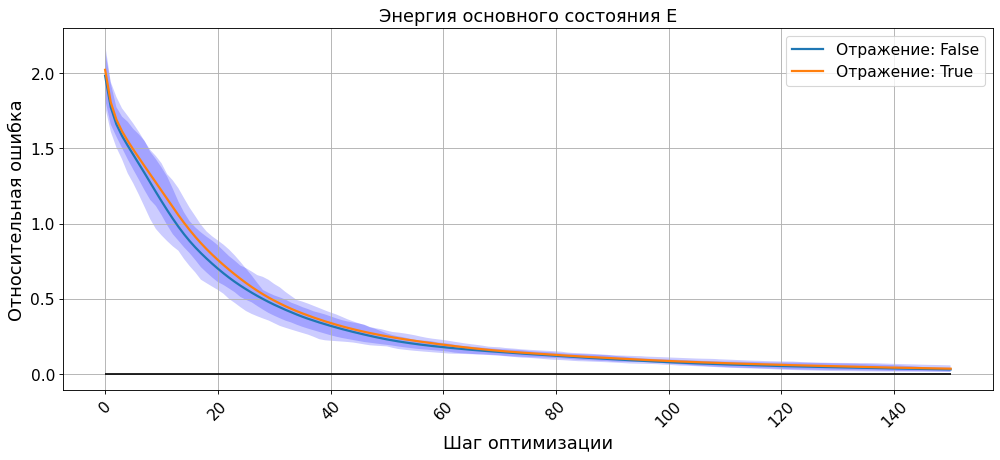
\includegraphics[width=\textwidth]{reflectance_comparence_3layers.png} а)}
\end{minipage}
\vfill
\begin{minipage}[H]{1.\linewidth}
\center{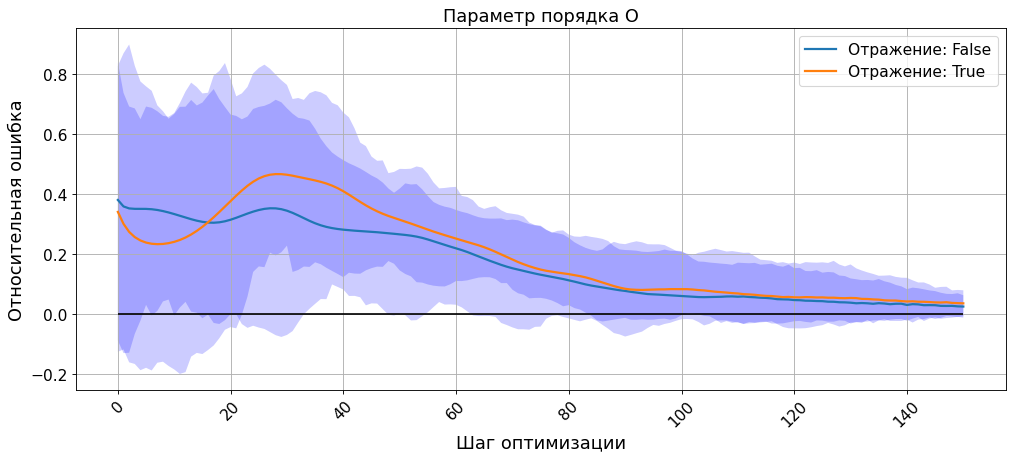
\includegraphics[width=\textwidth]{reflectance_comparence_O_3layers.png} б)}
\end{minipage}
\caption{Графики демонстрирует сравнение значений величин относительной ошибки расчета (а) энергии и (б) параметра порядка основного состояния гамильтониана Швингера размерности $N = 5$ в процессе оптимизации с использованием аппаратно-эффективного анзаца, основанного на двухкубитовых перепутывающих блоках $B_{RY}$, без блоков перемтановки каналов (синяя линия) и с блоком отражения каналов (оранжевая линия). Линии соответствуют зависимостям средних значений относительной ошибки оценки наблюдаемой на данной итерации за 50 запусков оптимизационного алгоритма со случайно выбранными начальными параметрами. Границы полупрозрачной области около линий соответствуют квантилям значений относительной ошибки оценки наблюдаемой на данной итерации за 50 запусков оптимизационного алгоритма со случайно выбранными начальными параметрами.}\label{fig:reflectance_comparence}
\end{figure}

\qquad На рис. \ref{fig:reflectance_comparence} продемонстрировано, что отличия при использовании отражающего блока между слоями укладываются в статистические погрешности проведённой серии измерений. При этом физическая реализация отражающего блока перестановок требует дополнительных ресурсов и вносит потери. Таким образом отражающий перестановочный блок оказывается нецелесообразным для использования.

\begin{figure}[H]
\begin{minipage}[H]{1.\linewidth}
\center{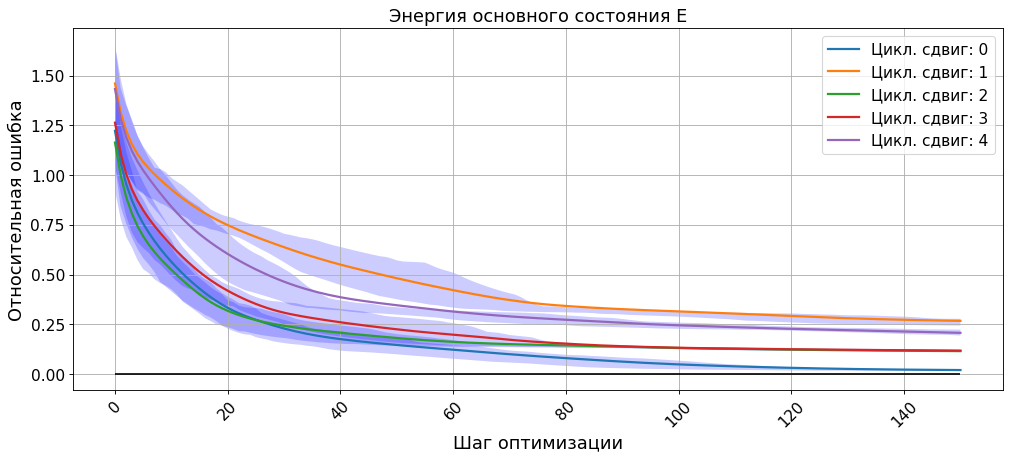
\includegraphics[width=\textwidth]{cycle_shift_comparence_2layers.png} а)}
\end{minipage}
\hfill
\begin{minipage}[H]{1.\linewidth}
\center{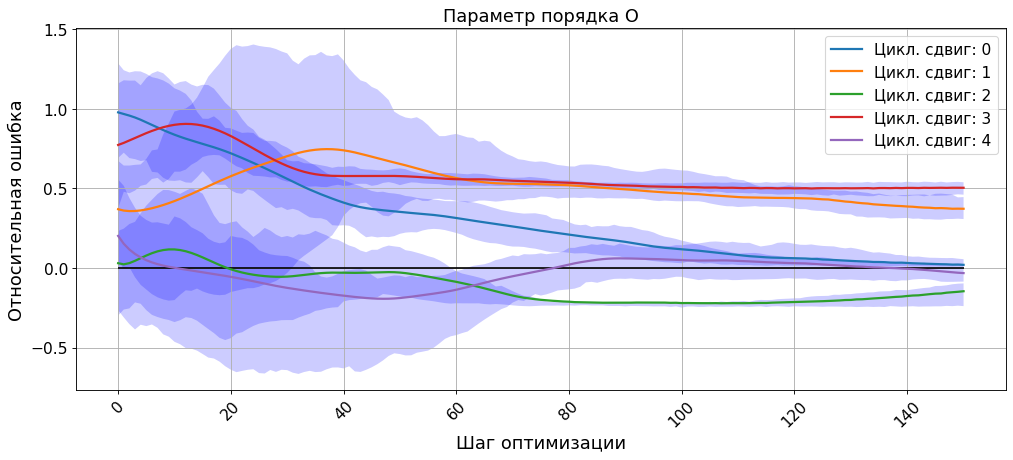
\includegraphics[width=\textwidth]{cycle_shift_comparence_O_2layers.png} б)}
\end{minipage}
\caption{Графики иллюстрируют сравнение значений величин относительной ошибки расчета (а) энергии и (б) параметра порядка основного состояния гамильтониана Швингера размерности $N = 5$ в процессе оптимизации с использованием аппаратно-эффективного анзаца, основанного на двухкубитовых перепутывающих блоках $B_{RY}$, с блоками различного циклического сдвига. Синяя, оранжевая, зелёная, красная и фиолетовая линии соответствуют циклическим сдвигам {0,1,2,3,4}.Линии соответствуют зависимостям средних значений относительной ошибки оценки наблюдаемой на данной итерации за 50 запусков оптимизационного алгоритма со случайно выбранными начальными параметрами. Границы полупрозрачной области около линий соответствуют квантилям значений относительной ошибки оценки наблюдаемой на данной итерации за 50 запусков оптимизационного алгоритма со случайно выбранными начальными параметрами.}\label{fig:shift_comparence}
\end{figure}

\qquad Применение циклического сдвига, помимо сложностей физической реализации, значительно снижает точность оценки основного состояния энергии (см. рис. \ref{fig:shift_comparence}), что делает его неэффективным в использовании.

\begin{figure}[H]
\begin{minipage}[H]{0.49\linewidth}
\center{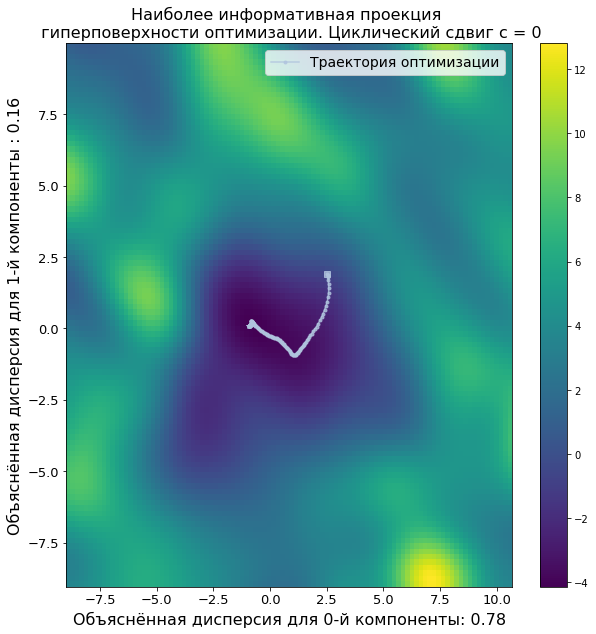
\includegraphics[width=\textwidth]{surface_c0_l3.png} a) Без перестановок}
\end{minipage}
\hfill
\begin{minipage}[H]{0.49\linewidth}
\center{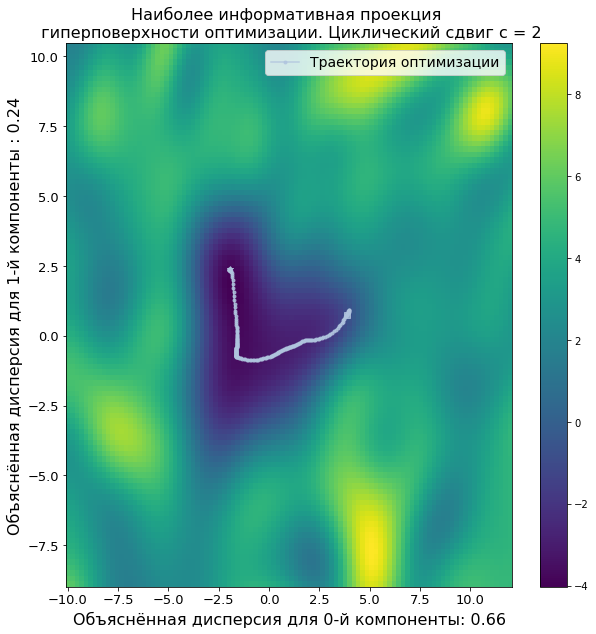
\includegraphics[width=\textwidth]{surface_c2_l3.png} б) Циклический сдвиг на 2 канала}
\end{minipage}
\caption{Иллюстрация демонстрирует сравнение наиболее информативных проекций гиперповерхности оптимизации соответствующей поиску энергии основного состояния гамильтониана Швингера размерности $N = 5$ c применением аппаратно-эффективного анзаца глубиной $l = 2$ слоя, основанного на двухкубитовом перепутывающем блоке $B_{RY}$, в зависимости от выбранного блока перестановки между слоями. Рассматриваются анзацы: а) без блоков перестановки между слоями и б) c блоком циклической перестановки на $с = 2$ канала.}\label{fig:proj_comp_permut}
\end{figure}

\qquad Снижение точности при использовании циклического блока перестановок может быть обосновано усложнением гиперповерхности оптимизации, что продемонстрировано на рис. \ref{fig:proj_comp_permut} визуально и подкреплено меньшей долей объяснённой дисперсии при оптимизации с использованием анзаца с циклическим сдвигом (94\% объяснённой дисперсии проекцией для случая без сдвига и 90\% для случая с циклическим сдвигом на $c = 2$ канала).

\subsection{Расчет энергии основного состояния молекул}


\qquad В данной работе для аппроксимации волновых функций молекул методом последовательных приближений Хартри-Фока используется готовая реализация соответствующих методов из библиотеки Openfermion-PySCF. Для представления гамильтониана в виде линейной комбинации строк матриц Паули используется встроенная реализация преобразований Джордана-Вигнера в библиотеке для квантовых вычислений PennyLane.

\qquad Моделирование поиска основного состояния двухатомных молекул проводится на молекулах $H_2$ и $LiH$. Активное пространство для $LiH$ ограничивается 2 орбиталями и 2 активными электронами, в приближении взаимодействия только электрона на внешней орбитали атома $Li$. Таким образом преобразования Джордана-Вигнера представляют фермионный гамильтониан в кубитовый размерности $N$ = 4.

\qquad Анализируется невязка оценки энергии основного состояния молекул для различного расстояния между атомами молекулы $d = 0.1, 0.2, \cdots , 3 \mathring A$. Для каждого фиксированного расстояния между атомами набирается статистика из 10 запусков процесса оптимизации и сравниваются финальные оценки энергии основного состояния c точными значениями.

\begin{figure}[H]
\begin{minipage}[H]{0.48\linewidth}
\center{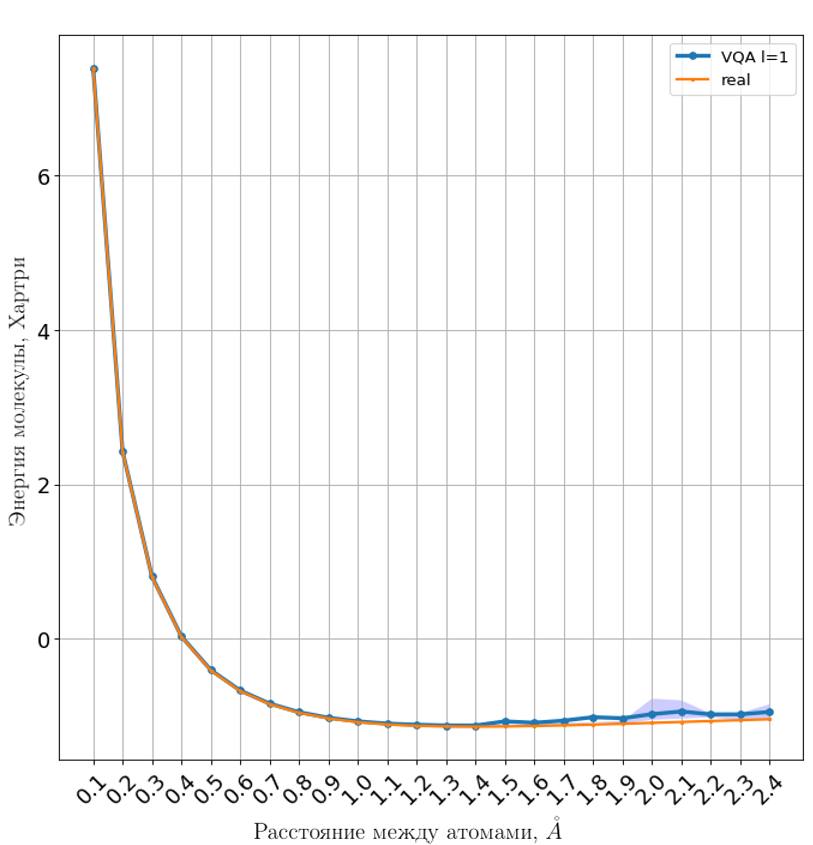
\includegraphics[width=\textwidth]{H2_dist_l1.png} а) Молекула $LiH$; слои $l = 1$}
\end{minipage}
\hfill
\begin{minipage}[H]{0.48\linewidth}
\center{\includegraphics[width=\textwidth]{H2_dist_l3.png} б) Молекула $H_2$; слои $l = 3$}
\end{minipage}
\vfill
\begin{minipage}[H]{0.48\linewidth}
\center{\includegraphics[width=\textwidth]{LiH_dist_l1.png} в) Молекула $LiH$; слои $l = 1$}
\end{minipage}
\hfill
\begin{minipage}[H]{0.48\linewidth}
\center{\includegraphics[width=\textwidth]{LiH_dist_l3.png} г) Молекула $LiH$; слои $l = 3$}
\end{minipage}
\caption{Графики иллюстрируют сравнение зависимостей расчитанной энергии основного состояния двухатомной молекулы с точным значением в зависимости от расстоянием между атомами молекулы. Рисунки а), б) иллюстрируют зависимости для молекулы $H_2$, а рисунки в), г) для молекулы $LiH$. Значения энергии основного состояния молекул расчитаны при помощи вариационного квантового алгоритма с использованием аппаратно-эффективного анзаца глубиной a),в) $l = 1$; б),г) $l = 3$ слоя без блоков перестановок с двухкубитовым перепутывающим блоком $B_{RY}$. Линии соответствуют зависимостям средних значений расчитанной наблюдаемой на данной итерации за 10 запусков ВКА. Границы полупрозрачной области около линий соответствуют квантилям значений рассчитанной наблюдаемой на данной итерации за 10 запусков оптимизационного процесса.}\label{fig:2atom_mols}
\end{figure}

\qquad Основные состояния молекул, как отмечалось ранее, часто характеризуются слабой запутанностью кубитов. Соответственно, предполагается, что достаточно точное описание можно получить даже с использованием однослойного анзаца, что продемонстрировано на рис. \ref{fig:2atom_mols}. Заметно, что для обеих молекул наблюдается хорошее совпадение оценки основного состояния с теоретическим значением для анзацев с глубиной $l = 1$ и $l = 3$.



\begin{figure}[H]
\begin{minipage}[H]{0.48\linewidth}
\center{\includegraphics[width=\textwidth]{LiH_Err_dist_l1.png} а) Невязка расчета энергии основного молекулы $LiH$ с использованием однослойного анзаца}
\end{minipage}
\hfill
\begin{minipage}[H]{0.48\linewidth}
\center{\includegraphics[width=\textwidth]{LiH_Err_dist_l3.png} б) Невязка расчета энергии основного молекулы $LiH$ с использованием анзаца глубиной $l = 3$ слоя}
\end{minipage}
\caption{Графики иллюстрируют сравнение зависимостей расчитанной энергии основного состояния двухатомной молекулы с точным значением от расстояния между атомами молекулы $LiH$. начения энергии основного состояния молекул расчитаны при помощи вариационного квантового алгоритма с использованием аппаратно-эффективного анзаца глубиной a) $l = 1$; б) $l = 3$ слоя без блоков перестановок с двухкубитовым перепутывающим блоком $B_{RY}$.}\label{fig:2atom_errs}
\end{figure}


\qquad Более подробное рассмотрение точности расчета энергии основного состояния для $LiH$ продемонстрировано на рис. \ref{fig:2atom_errs}. Заметно, что порядок относительной ошибки оценки основного состояния совпадает для анзацев с различной глубиной только для определённых расстояний между атомами молекулы, что указывает на ограниченность эффективного применения однослойных схем в задачах поиска основного состояния молекул.

\begin{figure}[H]
\begin{minipage}[H]{1.\linewidth}
\center{\includegraphics[width=\textwidth]{LiSH_fidelity.png}}
\end{minipage}
\caption{График иллюстрирует сравнение распределений невязки расчета энергии основного состояния трехатомной молекулы $H_2O$ с при помощи вариационного квантового алгоритма с использованием аппаратно-эффективного анзаца глубиной $l = 1$ и $l = 2$ слоя без блоков перестановок с двухкубитовым перепутывающими блоками $B_{RY}$.}\label{fig:3atom_errs}
\end{figure}

\qquad Аналогичные результаты можно получить и при рассмотрении трёхатомной молекулы $H_2O$. Вычислительные ресурсы, необходимые для моделирования процесса оптимизации трёхатомных молекул значительно больше, в связи с чем в данной работе проводится анализ невязки расчета энергии основного состояния молекулы с применением ВКА только для фиксированного состояния атомов молекулы, соответствующего оптимальной конфигурации. В оптимальной конфигурации расстояние между атомами водорода и кислорода $d = 0.9584 \mathring A$ а угол между атомами водорода $\alpha = 104.45^{\circ}$.

\qquad Для получения гамильтониана молекулы $H_2O$ использовано ограничение активного пространства в 4 орбитали. Далее в результате преобразования Джордана-Вигнера получен гамильтониан размерности $N = 8$ кубитов в форме линейной комбинации строк матриц Паули.

\qquad На рис. \ref{fig:3atom_errs} продемонстрировано, что невязка расчета энергии основного состояния молекулы $H_2O$ достаточна мала $\delta E \approx 10^{-4}$ в сравнении с химической точностью $\delta E_{chem} \approx 10^{-3}$ при использовании однослойнойного анзаца и практически не изменяется при увеличении глубины анзаца.

\qquad Таким образом однослойные анзацы представляются эффективными для оценки энергии основного состояния молекул, ввиду относительно простой масштабируемости физической реализации. 

\newpage

\begin{center}
\section*{ВЫВОДЫ}
\end{center}

\addcontentsline{toc}{section}{ВЫВОДЫ}

\qquad В данной работе исследовано применение эффективно реализуемых физически квантовых схем в качестве анзаца для вариационных квантовых алгоритмов, в ходе которого:

\begin{itemize}

\item Рассмотрены различные конфигурации аппаратно-эффективного анзаца. Проведено сравнение 4-х видов двухкубитового перепутывающего блока, перестановки каналов между слоями анзаца путём отражения и циклического сдвига;

\item Проведён анализ эффективности вариационного алгоритма в зависимости от глубины аппаратно-эффективного анзаца;

\item Исследована гиперповерхность оптимизации для различных конфигураций анзаца;

\item Проведён анализ эффективности применения вариационных квантовых алгоритмов на основе аппаратно-эффективного анзаца различной конфигурации для задач поиска энергии основного состояния гамильтониана Швингера различной размерности и гамильтонианов молекул $H_2$, $LiH$, $H_2O$. 

\end{itemize}


\qquad Результаты дипломной работы:

\begin{itemize}

\item Найдена оптимальная из рассмотренных конфигураций аппаратно-эффективного анзаца. Установлено, что рассмотренные блоки перестановки каналов увеличивают относительную ошибку оценки основного состояния энергии в результате усложнения гиперповерхности оптимизации и не целесообразны к использованию. Установлено, что наилучшая точность оценки энергии основного состояния достигается с использованием в качестве двухкубитового запутывающего блока наименее экспрессивного $B_{RY}$.

\item Установлено, что для поиска энергии основного состояния произвольного гамильтониана  однослойный аппаратно-эффективный анзац демонстрирует низкую точность, что вероятно связано с узким классом приготавливаемых состояний, и сложностями приготовления сильно запутанного состояний ввиду одномерной геометрии связей. При этом для оценки энергии основного состояния рассмотренных молекул однослойная схема демонстрирует высокую точность, что вероятно связано с малой степенью запутанности основных состояний рассмотренных молекул.

\item Продемонстрировано, что многослойный аппаратно-эффективный анзац решает рассмотренные задачи с высокой точностью.

\item В процессе моделирования поиска энергии основного состояния молекул при помощи вариационного квантового алгоритма на основе аппаратно-эфективного анзаца с точностью $10^{-4}$ Хартри, превосходящей химическую точность $10^{-3}$ Хартри, найдены энергии основных состояний двухатомных молекул $LiH$ и $H_2$ для межатомных расстояний $d = 0.1, 0.2, \cdots , 3 \mathring A$ и трёхатомной молекулы $H_2O$ в оптимальной конфигурации, соответствующей расстоянию между атомами водорода и кислорода $d = 0.9584 \mathring A$ и углу между атомами водорода $\alpha = 104.45^{\circ}$.
\end{itemize}

\newpage

\addcontentsline{toc}{section}{СПИСОК ИСПОЛЬЗОВАННЫХ ИСТОЧНИКОВ}

\bibliography{library}


\end{document}